\documentclass[aspectratio=169, 10pt]{beamer}

% Theme and Color Settings
\usetheme{Madrid}
\usecolortheme{whale}
\usefonttheme{professionalfonts}

% Packages
\usepackage{graphicx}
\usepackage{booktabs}
\usepackage{tikz}
\usepackage{caption}
\usepackage{hyperref}
\usepackage{longtable}
\usepackage{tabularx}
\usepackage{array}
\usepackage{multirow}
\usepackage{adjustbox}

% Customization
\setbeamertemplate{navigation symbols}{}
\setbeamertemplate{caption}[numbered]
\setbeamertemplate{footline}[frame number]

% Custom column types
\newcolumntype{Y}{>{\raggedright\arraybackslash}X}
\newcolumntype{Z}{>{\centering\arraybackslash}X}

% Title Information
\title[Veritas: AI Enhanced Assessment]{Veritas: AI Enhanced Online Assessment and Monitoring System}
\subtitle{Final Year Project Report Presentation}
\author[Team Veritas]{
    \textbf{Team Members:} \\
    Abraham Mulugeta (ETS0107/14) \and Alazar Gebre (ETS0132/14) \\
    Tadiyos Dejene (ETS1522/14) \and Tamirat Dejene (ETS1518/14) \\
    Yohannes Tigistu (ETS1703/14) \\
    \vspace{0.3cm}
    \textbf{Advisor:} Mr. Muleta Taye (PhD)
}
\institute[AASTU]{
    Department of Software Engineering \\
    College of Engineering \\
    Addis Ababa Science and Technology University
}
\date{January 2026}

% Logo
\titlegraphic{
\includegraphics[width=2.5cm]{assets/aastu_logo.jpg}}

\begin{document}

% =============================================================================
% TITLE SLIDE
% =============================================================================
\begin{frame}
    \titlepage
\end{frame}

% =============================================================================
% TABLE OF CONTENTS
% =============================================================================
\begin{frame}{Presentation Outline}
    \tableofcontents
\end{frame}

% =============================================================================
% SECTION 1: INTRODUCTION
% =============================================================================
\section{Introduction}

% =============================================================================
% Background
% =============================================================================
\begin{frame}{Background: Digital Transformation in Assessment}
    \begin{block}{Global Context}
        \begin{itemize}
            \item Rapid transition from paper-based to digital assessments worldwide
            \item Accelerated by need for efficiency, scalability, and immediate feedback
            \item Remote evaluation technologies reduce logistical overhead
            \item Better geographical reach and automated grading capabilities
        \end{itemize}
    \end{block}
    
    \begin{block}{Ethiopian Context}
        \begin{itemize}
            \item Significant growth in online examination platforms
            \item Adoption in education and organizational recruitment sectors
            \item Current implementations: Generic platforms or manual processes
            \item Not aligned with local infrastructure (internet stability, institutional requirements)
        \end{itemize}
    \end{block}
\end{frame}

\begin{frame}{The Integrity Challenge}
    \begin{columns}
        \column{0.5\textwidth}
        \textbf{The Core Problem}
        \begin{itemize}
            \item Convenience of remote testing is undeniable
            \item Ensuring genuine candidate performance is challenging
            \item Growing demand for objective talent evaluation
            \item Need for high trust without prohibitive costs
        \end{itemize}
        
        \column{0.5\textwidth}
        \textbf{Veritas Solution}
        \begin{itemize}
            \item Modern web technologies + AI
            \item Bridge global standards \& local needs
            \item Locally developed, secure platform
            \item Data sovereignty priority
            \item Operational efficiency focus
        \end{itemize}
    \end{columns}
    
    \vspace{0.5cm}
    \begin{center}
        \textit{Contributing to technological independence and digital innovation in Ethiopia}
    \end{center}
\end{frame}

% =============================================================================
% Problem Statement
% =============================================================================
\begin{frame}{Statement of the Problem (1/3)}
    \begin{alertblock}{Data Sovereignty \& Dependency Issues}
        \begin{itemize}
            \item Organizations depend on foreign-hosted solutions (TestGorilla, HackerRank, ProctorU)
            \item \textbf{High subscription costs} in foreign currency (strictly regulated in Ethiopia)
            \item \textbf{Data stored abroad} - violates Digital Ethiopia 2030 Strategy
            \item Lack of integration with local identity infrastructures
            \item Ministry of Innovation and Technology (2025): Need for ``Digital Sovereignty''
        \end{itemize}
    \end{alertblock}
\end{frame}

\begin{frame}{Statement of the Problem (2/3)}
    \begin{alertblock}{Manual Grading Bottleneck}
        \begin{itemize}
            \item Existing tools limited to automating \textbf{objective assessments only}
            \item Subjective evaluations (essays, descriptive answers) remain manual
            \item Labor-intensive process with significant delays
            \item Introduces human bias in grading
            \item Organizations forced to choose: simplicity of MCQ OR inefficiency of manual review
            \item No automated framework for high-volume subjective submissions
        \end{itemize}
    \end{alertblock}
\end{frame}

\begin{frame}{Statement of the Problem (3/3)}
    \begin{alertblock}{Infrastructure \& Accessibility Barriers}
        \begin{itemize}
            \item Global platforms (TestGorilla, ProctorU) optimized for high-bandwidth, stable internet
            \item Ethiopian context: High latency, connectivity fluctuations common
            \item Results in session timeouts and data loss
            \item Compromises assessment reliability
            \item \textbf{Critical challenges:}
            \begin{itemize}
                \item Maintaining examination credibility
                \item Preventing cheating
                \item Verifying identity
                \item Handling large-scale automated assessments
            \end{itemize}
        \end{itemize}
    \end{alertblock}
    
    \vspace{0.3cm}
    \begin{center}
        \textbf{Need:} Secure, intelligent platform tailored to Ethiopian organizations
    \end{center}
\end{frame}

% =============================================================================
% Objectives
% =============================================================================
\begin{frame}{Objectives}
    \begin{block}{General Objective}
        To design and develop an \textbf{AI-enhanced online assessment and monitoring system}
    \end{block}
    
    \begin{block}{Specific Objectives (1/2)}
        \begin{enumerate}
            \item Gather and analyze user and organization requirements
            \item Design multi-tenant architecture for independent examination environments
            \item Implement secure authentication (enterprise IDs/unique tokens)
            \item Authenticate real identity through face recognition models
            \item Develop intelligent monitoring (tab-switch, mouse tracking, IP tracking)
        \end{enumerate}
    \end{block}
\end{frame}

\begin{frame}{Specific Objectives (2/2)}
    \begin{block}{Specific Objectives (continued)}
        \begin{enumerate}
            \setcounter{enumi}{5}
            \item Integrate automated and manual grading mechanisms
            \item Build customizable enterprise dashboard for exam management
            \item Design and generate organization-specific certificates
            \item Integrate payment and subscription management (Basic, Premium, Enterprise)
            \item Evaluate system's usability, scalability, accuracy, and security
            \item Deploy functional prototype in controlled environment
        \end{enumerate}
    \end{block}
\end{frame}

% =============================================================================
% Scope and Limitations
% =============================================================================
\begin{frame}{Scope of the Project}
    \textbf{Focus:} Design, development, and evaluation of a \textit{prototype} AI-enhanced system
    
    \begin{block}{What's Included}
        \begin{itemize}
            \item Multi-tenant system architecture design
            \item Core examination management (creation, scheduling, participation)
            \item Basic authentication (enterprise credentials/tokens)
            \item AI-assisted smart proctoring (tab-switch, mouse tracking, image capture)
            \item Automated grading for objective \& essay-based questions
            \item Role-based administrative dashboards
            \item Simulation of subscription-based access control
        \end{itemize}
    \end{block}
    
    \begin{alertblock}{What's Excluded}
        Full-scale production deployment, large-scale real-world usage, legal compliance certification, continuous maintenance, production-level payment processing
    \end{alertblock}
\end{frame}

\begin{frame}{Limitations}
    \begin{block}{Technical \& Contextual Limitations}
        \begin{description}
            \item[Platform] Web application only (no mobile/desktop apps)
            \item[Biometric] No fingerprint or voice verification (hardware/privacy constraints)
            \item[Human Proctoring] Automated only (no real-time human invigilation via video)
            \item[AI Models] Lightweight, pre-trained models - accuracy varies with lighting, camera quality
            \item[Dataset] Limited diversity in training data
            \item[Scalability] Nationwide deployment beyond current scope
        \end{description}
    \end{block}
    
    \vspace{0.3cm}
    \textit{Future iterations may address these limitations}
\end{frame}

% =============================================================================
% Methodology
% =============================================================================
\begin{frame}{Methodology: Agile Scrum Framework}
    \begin{columns}
        \column{0.5\textwidth}
        \textbf{Why Agile?}
        \begin{itemize}
            \item AI-driven, security-critical system
            \item Continuous refinement needed
            \item Complex proctoring layers
            \item Semantic analysis requirements
            \item Rapid stakeholder feedback
            \item Adapt to Ethiopian infrastructure
        \end{itemize}
        
        \column{0.5\textwidth}
        \textbf{Key Benefits}
        \begin{itemize}
            \item Iterative development cycles
            \item Early risk mitigation
            \item Network bottleneck validation
            \item AI false-positive detection
            \item User-centered design
            \item Traceability \& quality
        \end{itemize}
    \end{columns}
    
    \vspace{0.5cm}
    \begin{center}
        \textbf{Two Components:} Research \& Requirements Engineering + System Development Process
    \end{center}
\end{frame}

\begin{frame}{Research and Requirements Engineering}
    \begin{block}{A. Interviews with HRs and Educators}
        \textbf{Focus:} Administrative and pedagogical needs
        \begin{itemize}
            \item Average turnaround time for subjective grading
            \item Specific cheating behaviors difficult to detect remotely
            \item Data sovereignty criticality
            \item Common technical complaints from candidates
        \end{itemize}
    \end{block}
    
    \begin{block}{B. Literature Review}
        \textbf{Focus:} Academic papers, technical docs, industry reports
        \begin{itemize}
            \item State-of-the-art benchmarks for Transformer-based grading
            \item Trade-off between strict proctoring and privacy
            \item Vulnerabilities in process-level isolation
            \item Best practices for high-latency WebSocket communication
        \end{itemize}
    \end{block}
\end{frame}

\begin{frame}{Research Methods (continued)}
    \begin{block}{C. Observational Studies of Existing Tools}
        \textbf{Focus:} Hands-on comparative analysis (ProctorU, TestGorilla, local systems)
        \begin{itemize}
            \item Failure points on typical 3G/4G Ethiopian networks
            \item Administrator workflow complexity
            \item System response to local hardware constraints
            \item Proctoring false positives in local testing environments
        \end{itemize}
    \end{block}
    
    \begin{block}{Comparative Analysis Outcomes}
        \begin{itemize}
            \item \textbf{Global tools:} High costs, lack of localized support
            \item \textbf{Local platforms:} Limited scalability, minimal AI capabilities
            \item \textbf{User concerns:} Intrusiveness, false-positive rates
        \end{itemize}
    \end{block}
\end{frame}

% =============================================================================
% System Development Process
% =============================================================================
\begin{frame}{System Development Life Cycle (SDLC)}
    \begin{description}
        \item[Phase 1: Planning] Define scope, technical feasibility, finalize product backlog, prioritize MVP features (GitHub Projects, Trello)
        
        \item[Phase 2: Design] Event-driven microservices architecture (choreography-based), handle high-volume proctoring events asynchronously (Visual Paradigm, Figma)
        
        \item[Phase 3: Implementation] Hybrid stack (Go for concurrency, FastAPI/Python for AI), facial recognition with liveness, React SPA, PostgreSQL
        
        \item[Phase 4: QA \& Testing] Unit tests (PyTest, Go Test, Jest), scalability testing (JMeter - 500+ concurrent users), security red teaming (95\% detection target)
        
        \item[Phase 5: Documentation] Swagger/OpenAPI, JSDoc, system manuals with local-network troubleshooting
    \end{description}
\end{frame}

\begin{frame}{Technology Stack Details}
    \begin{columns}
        \column{0.5\textwidth}
        \textbf{Backend Services}
        \begin{itemize}
            \item \textbf{Go (Golang):} Real-time proctoring event streamer, API gateway
            \item \textbf{Python/FastAPI:} AI services (subjective grading, anomaly detection)
            \item \textbf{PostgreSQL:} ACID guarantees
        \end{itemize}
        
        \column{0.5\textwidth}
        \textbf{Frontend \& AI}
        \begin{itemize}
            \item \textbf{React:} SPA for dashboard, real-time handling
            \item \textbf{OpenCV/DeepFace:} Facial recognition with liveness
            \item \textbf{Transformers:} NLP for essay grading
        \end{itemize}
    \end{columns}
    
    \vspace{0.5cm}
    \begin{center}
        
\includegraphics[width=0.6\textwidth]{assets/aastu_logo.jpg}
    \end{center}
\end{frame}

% =============================================================================
% Significance
% =============================================================================
\begin{frame}{Significance of the Study}
    \begin{block}{Academic Contribution}
        \begin{itemize}
            \item Demonstrates robust AI-enhanced monitoring with resource-efficient engineering
            \item Microservices architecture combining Go concurrency + Python analytics
            \item Continuous identity verification + semantic AI grading
            \item Blueprint for scalable, fair evaluation systems
            \item Beyond keyword matching to contextual understanding
        \end{itemize}
    \end{block}
    
    \begin{block}{Practical Benefits}
        \begin{itemize}
            \item \textbf{For HR \& Admins:} Streamlined evaluation, reduced bias, lower costs
            \item \textbf{For Candidates:} Fair, transparent, low-latency testing environment
            \item \textbf{For Ethiopia:} Digital sovereignty, technological independence
        \end{itemize}
    \end{block}
\end{frame}

\begin{frame}{Report Structure Overview}
    \begin{description}
        \item[Chapter 1: Introduction] Background, problem statement, objectives, scope, methodology
        \item[Chapter 2: Literature Review] Existing systems, smart proctoring, AI-based monitoring, gaps
        \item[Chapter 3: Methodology] Requirements analysis, system architecture, design specifications
        \item[Chapter 4: Design \& Implementation] Development process, technologies, core modules
        \item[Chapter 5: Testing \& Evaluation] Performance, accuracy, usability, security testing
        \item[Chapter 6: Conclusion] Key findings, contributions, future work recommendations
    \end{description}
\end{frame}


% =============================================================================
% SECTION 2: LITERATURE REVIEW
% =============================================================================
\section{Literature Review}

% =============================================================================
% Overview
% =============================================================================
\begin{frame}{Literature Review: Overview}
    \begin{block}{Focus Areas}
        Critical review of literature concerning:
        \begin{itemize}
            \item Online assessment systems evolution (COVID-19 pandemic impact)
            \item Online proctoring and integrity assurance
            \item AI-driven Automated Essay Scoring (AES)
            \item Large Language Models (LLMs) in assessment
            \item Natural Language Processing (NLP) advancements
        \end{itemize}
    \end{block}
    
    \begin{block}{Key References}
        \begin{itemize}
            \item Topuz (2022): Systematic review of 22 online assessment systems
            \item Hussein (2020): Commercial proctoring tools evaluation
            \item Mizumoto \& Eguchi (2023): GPT-3 for AES
            \item Schneider (2024): GPT-4 for short answer grading
        \end{itemize}
    \end{block}
\end{frame}

% =============================================================================
% Evolution Phases
% =============================================================================
\begin{frame}{Evolution of Online Assessment Systems}
    \begin{table}[]
        \centering
        \small
        \begin{tabular}{l p{8cm}}
            \toprule
            \textbf{Phase} & \textbf{Key Characteristics} \\
            \midrule
            \textbf{Phase 1} & \textbf{Manual Online (Pre-2020):} Basic digital delivery, webcam monitoring, \\
            (Pre-2020) & browser lockdowns. Limited real-world deployment. \\
            \midrule
            \textbf{Phase 2} & \textbf{Emergency Remote Teaching (2020-2021):} Rapid adoption, \\
            (2020-2021) & desktop-focused, facial recognition, semi-automatic monitoring, \\
            & LMS integration (Moodle). Infrastructure gaps exposed. \\
            \midrule
            \textbf{Phase 3} & \textbf{AI Integration (2021-2024):} Machine learning for cheating \\
            (2021-2024) & detection, real-time monitoring, deep learning for behavior analysis. \\
            & Issues: false positives, bias concerns. \\
            \midrule
            \textbf{Phase 4} & \textbf{User-Centric \& Ethics (2024-2025):} Privacy focus, GDPR \\
            (2024-2025) & compliance, hybrid models, human oversight, equity considerations. \\
            \midrule
            \textbf{Phase 5} & \textbf{LLM-Driven Scoring (2023-2026):} GPT-3/4, ChatGPT, Llama \\
            (2023-2026) & for AES and ASAG. Rubric-based evaluation, feedback generation. \\
            \bottomrule
        \end{tabular}
    \end{table}
\end{frame}

% =============================================================================
% Study Related Works
% =============================================================================
\begin{frame}{Key Related Works (1/3)}
    \begin{block}{Topuz et al. (2022) - Systematic Review}
        \begin{itemize}
            \item Reviewed 22 online assessment systems during Emergency Remote Teaching
            \item \textbf{Major features identified:}
            \begin{itemize}
                \item Multi-platform compatibility
                \item Enhanced security (biometric authentication)
                \item Automated proctoring
            \end{itemize}
            \item Commercial systems: Examity, ProctorU, Safe Exam Browser
            \item Multimodal authentication: webcam, keystroke analysis, facial recognition
        \end{itemize}
    \end{block}
\end{frame}

\begin{frame}{Key Related Works (2/3)}
    \begin{block}{Kurniati et al. (2023) - Indonesian Context}
        \begin{itemize}
            \item Challenges: Infrastructure limitations, academic dishonesty, inconsistent discipline
            \item \textbf{Adaptive strategies:} Shift to subjective assessments, home visits, shared mobile access
        \end{itemize}
    \end{block}
    
    \begin{block}{Hussein (2020) \& Arno (2021)}
        \begin{itemize}
            \item \textbf{Hussein:} Cost, accessibility, ethical concerns as barriers
            \item \textbf{Arno:} Compared 29 commercial systems
            \item \textbf{Conclusion:} Hybrid approaches (automated + human) optimal for integrity \& UX
        \end{itemize}
    \end{block}
\end{frame}

\begin{frame}{Key Related Works (3/3)}
    \begin{block}{AI-Based Proctoring}
        \begin{itemize}
            \item \textbf{Jia \& He (2021):} IOPS - facial, eye, voice monitoring. Reduced cheating in university exams
            \item \textbf{Rahim (2020):} Guidelines for effective online assessment during ERT
            \item \textbf{Ali (2025):} Phased implementation in medical education. Mock exams improved confidence
        \end{itemize}
    \end{block}
    
    \begin{block}{LLM-Based Grading}
        \begin{itemize}
            \item \textbf{Mizumoto \& Eguchi (2023):} GPT-3 for TOEFL essays (QWK $\sim$0.7)
            \item \textbf{Schneider (2024):} GPT-4 for short answers - reliable on rubric-based benchmarks
            \item \textbf{Mansour (2024):} LLMs for proficiency scoring with trait-based feedback
            \item \textbf{Kundu (2024):} LLMs harsher on nuanced responses, useful as assistants
        \end{itemize}
    \end{block}
\end{frame}

% =============================================================================
% Milestones
% =============================================================================
\begin{frame}{Milestones: Phase 1 \& 2}
    \begin{block}{Phase 1: Manual Online Assessments (Pre-2020)}
        \textbf{Strengths:}
        \begin{itemize}
            \item Clear conceptual frameworks for design and security
            \item Authentication classification (knowledge, possession, biometric, contextual)
        \end{itemize}
        \textbf{Limitations:}
        \begin{itemize}
            \item Largely descriptive, limited real-world testing
            \item Minimal emphasis on scalability or low-bandwidth environments
        \end{itemize}
    \end{block}
    
    \begin{block}{Phase 2: Emergency Remote Teaching (2020-2021)}
        \textbf{Strengths:}
        \begin{itemize}
            \item Comprehensive overview of pandemic-driven solutions
            \item Desktop-focused, pre-exam facial recognition, LMS integration
        \end{itemize}
        \textbf{Limitations:}
        \begin{itemize}
            \item Self-reported data, overlooks infrastructure constraints in developing regions
        \end{itemize}
    \end{block}
\end{frame}

\begin{frame}{Milestones: Phase 3, 4 \& 5}
    \begin{block}{Phase 3: AI \& Automation (2021-2024)}
        \textbf{Strengths:} Proactive, automated integrity enforcement \\
        \textbf{Limitations:} Requires high-quality data, stable internet; bias, fairness, privacy concerns
    \end{block}
    
    \begin{block}{Phase 4: User-Centric Design (2024-2025)}
        \textbf{Strengths:} Ethics, privacy, GDPR compliance, human oversight \\
        \textbf{Limitations:} Early stages, limited empirical evidence, Western-centric
    \end{block}
    
    \begin{block}{Phase 5: LLM-Driven Scoring (2023-2026)}
        \textbf{Strengths:} Scalability, personalization, instant feedback (QWK 0.68-0.88) \\
        \textbf{Limitations:} Prompt design sensitivity, training biases, variable correlations, limited validation in resource-constrained environments
    \end{block}
\end{frame}

% =============================================================================
% Gaps Identified
% =============================================================================
\begin{frame}{Critical Gaps Identified (1/3)}
    \begin{alertblock}{1. Poor Accessibility for Students with Disabilities}
        \begin{itemize}
            \item Restrictive security measures (browser lockdowns, hidden taskbars)
            \item Exclude users dependent on assistive technologies
            \item Lack of Universal Design for Learning (UDL) principles
            \item Inconsistent accessibility policies across institutions
            \item \textbf{Design bias:} Security \& standardization over inclusivity
        \end{itemize}
    \end{alertblock}
\end{frame}

\begin{frame}{Critical Gaps Identified (2/3)}
    \begin{alertblock}{2. The ``Security vs. Connectivity'' Gap}
        \begin{itemize}
            \item Secure proctoring requires continuous high-speed internet
            \item Weak digital infrastructure in developing regions
            \item Indonesian teachers abandoned video-based testing (Kurniati 2023)
            \item 57\% of Pakistani medical students experienced internet instability (Ali 2025)
            \item Commercial tools require intensive data streaming, high computing power
            \item \textbf{Missing:} Adaptive, low-bandwidth monitoring mechanisms
        \end{itemize}
    \end{alertblock}
    
    \begin{alertblock}{3. The ``Intelligent Proctoring'' Gap}
        \begin{itemize}
            \item Polarization: Simple unproctored tools vs. costly AI-driven systems
            \item High-end platforms financially inaccessible to smaller universities
            \item \textbf{Missing:} Accessible ``Passive AI'' solutions (tab-switch detection, periodic image capture, local face verification)
        \end{itemize}
    \end{alertblock}
\end{frame}

\begin{frame}{Critical Gaps Identified (3/3)}
    \begin{alertblock}{4. The ``Local Customization'' Gap}
        \begin{itemize}
            \item Technologies developed for Western institutions
            \item Seldom consider local privacy laws, language interfaces, workflows
            \item Nearly all systems hosted abroad
            \item Difficulties adapting foreign platforms to local realities
            \item \textbf{Missing:} Indigenous, region-specific frameworks compliant with national data protection (e.g., Ethiopia's Personal Data Protection Proclamation)
        \end{itemize}
    \end{alertblock}
    
    \begin{alertblock}{5. ASAG \& AES Gaps}
        \begin{itemize}
            \item \textbf{ASAG:} Variable GPT-4 performance, inconsistent domain-specific scoring
            \item \textbf{AES:} Variable human-LLM agreement, harsher on nuanced essays, limited non-English/technical domain adaptation
        \end{itemize}
    \end{alertblock}
\end{frame}

% =============================================================================
% Lessons Learned
% =============================================================================
\begin{frame}{Lessons Learned from Literature}
    \begin{enumerate}
        \item \textbf{Infrastructure \& Inclusivity Matter}
        \begin{itemize}
            \item Digital divide's role in exam integrity
            \item Flexible system design for varying connectivity
        \end{itemize}
        
        \item \textbf{Ethical \& Data-Conscious Design}
        \begin{itemize}
            \item Transparent data handling, user-centric approaches
        \end{itemize}
        
        \item \textbf{Integrity Cannot Rely on Trust Alone}
        \begin{itemize}
            \item Technical methods essential (tab-switching, face detection)
            \item Changing question types insufficient without supervision
        \end{itemize}
        
        \item \textbf{Infrastructure is Primary Constraint}
        \begin{itemize}
            \item Technical failures most frequent complaint
            \item Client-side AI processing crucial for unstable connections
        \end{itemize}
        
        \item \textbf{User Experience Impacts Performance}
        \begin{itemize}
            \item Complex interfaces increase anxiety and errors
            \item Intuitive portals with minimal setup required
        \end{itemize}
    \end{enumerate}
\end{frame}

\begin{frame}{Lessons Learned (continued)}
    \begin{enumerate}
        \setcounter{enumi}{5}
        \item \textbf{LLM Consistency}
        \begin{itemize}
            \item Reliable, generalizable scoring across large datasets
            \item Outperforms traditional methods in efficiency
        \end{itemize}
        
        \item \textbf{Human-AI Collaboration}
        \begin{itemize}
            \item Dual-process models enhance accuracy
            \item LLMs as assistants, not standalone tools
        \end{itemize}
        
        \item \textbf{Prompting Techniques}
        \begin{itemize}
            \item Zero-shot and chain-of-thought prompting improve rubric-based evaluation
            \item Better handling of subjective criteria
        \end{itemize}
    \end{enumerate}
    
    \vspace{0.5cm}
    \begin{center}
        \textbf{These lessons directly inform Veritas design decisions}
    \end{center}
\end{frame}


% =============================================================================
% SECTION 3: PROBLEM ANALYSIS AND MODELING
% =============================================================================
\section{Problem Analysis and Modeling}

% =============================================================================
% Existing System Overview
% =============================================================================
\begin{frame}{Existing Systems in Ethiopia}
    \begin{block}{Foreign-Hosted Commercial Platforms}
        \begin{description}
            \item[TestGorilla] Pre-built assessments (coding, cognitive, personality), automated grading, basic webcam proctoring
            \item[HackerRank] Technical evaluations, coding challenges, real-time compilation, plagiarism detection
            \item[ProctorU] Live proctoring, human invigilators + AI tools, eye-tracking, screen recording
        \end{description}
    \end{block}
    
    \begin{block}{Local Alternatives}
        \begin{itemize}
            \item \textbf{Moodle:} Open-source LMS, timed quizzes, MCQ, browser lockdowns
            \item \textbf{Google Forms:} Basic quiz administration
            \item \textbf{Manual Processes:} Paper-based or hybrid (email + manual grading)
            \item \textbf{Enterprise Tools:} LinkedIn Assessments, custom spreadsheets
        \end{itemize}
    \end{block}
    
    \textit{Typical architecture: Client-server model, cloud storage (AWS/Google Cloud), limited local identity integration}
\end{frame}

% =============================================================================
% Problems - Technical
% =============================================================================
\begin{frame}{Identified Problems: Technical Limitations}
    \begin{alertblock}{(a) Infrastructure Incompatibility}
        \begin{itemize}
            \item Foreign platforms optimized for high-bandwidth, stable internet
            \item Ethiopian context: 50-100ms latency, common outages (Ethio Telecom)
            \item Results: Session timeouts, data loss, degraded proctoring quality
            \item Example: ProctorU live streaming fails on 3G/4G networks
        \end{itemize}
    \end{alertblock}
    
    \begin{alertblock}{(b) Lack of Automated Subjective Grading}
        \begin{itemize}
            \item Current systems excel at objective assessments (MCQ)
            \item Manual grading for essays and open-ended questions
            \item Creates bottlenecks: turnaround times extend to days/weeks
            \item Impacts recruitment cycles (HR manager interviews)
        \end{itemize}
    \end{alertblock}
    
    \begin{alertblock}{(c) Weak Integration with Local Systems}
        \begin{itemize}
            \item No linkage with Ethiopian National ID or enterprise directories
            \item Authentication defaults to username/password
            \item Increases vulnerability to identity spoofing
        \end{itemize}
    \end{alertblock}
\end{frame}

% =============================================================================
% Problems - Economic & Operational
% =============================================================================
\begin{frame}{Identified Problems: Economic \& Operational}
    \begin{alertblock}{(d) Economic Limitations}
        \begin{itemize}
            \item \textbf{High subscription costs:} Foreign currency (USD) required
            \item Regulated and scarce in Ethiopia
            \item Annual fees exceed ETB 500,000 for enterprise plans
            \item Inaccessible to small institutions and startups
            \item \textbf{External hosting dependency:} Ongoing costs, compliance risks
        \end{itemize}
    \end{alertblock}
    
    \begin{alertblock}{(e) Operational Limitations}
        \begin{itemize}
            \item \textbf{Cheating vulnerabilities:} Basic proctoring insufficient for sophisticated behaviors
            \item False positives in AI monitoring (poor lighting, device quality)
            \item \textbf{Scalability issues:} Moodle struggles beyond 500 concurrent users
            \item Crashes during peak times
            \item \textbf{UX \& accessibility gaps:} No localization (Amharic), restrictive features exclude disabled users
        \end{itemize}
    \end{alertblock}
\end{frame}

% =============================================================================
% Problems - Ethical & Regulatory
% =============================================================================
\begin{frame}{Identified Problems: Ethical \& Regulatory}
    \begin{alertblock}{(f) Ethical and Regulatory Limitations}
        \begin{description}
            \item[Data Sovereignty] Storing data abroad violates Digital Ethiopia 2030 Strategy. Exposes data to foreign jurisdiction and potential breaches.
            
            \item[Bias \& Privacy] AI components introduce biases (inaccurate facial recognition for diverse ethnicities). Privacy concerns without clear compliance to Ethiopia's Personal Data Protection Proclamation.
            
            \item[Limited Customization] No multi-tenant environments for multiple organizations. No automated certificate generation. No local payment system support (Telebirr).
        \end{description}
    \end{alertblock}
    
    \vspace{0.5cm}
    \begin{center}
        \textbf{These problems underscore the need for Veritas}
    \end{center}
\end{frame}


% =============================================================================
% SECTION 4: SYSTEM REQUIREMENTS
% =============================================================================
\section{System Requirements Specification}

% =============================================================================
% Requirements Overview
% =============================================================================
\begin{frame}{Requirements Specification Overview}
    \begin{block}{Requirement Categorization}
        \textbf{Naming Convention:}
        \begin{itemize}
            \item \textbf{FR-[CATEGORY]-[NNN]} for functional requirements
            \item \textbf{NFR-[CATEGORY]-[NNN]} for non-functional requirements
            \item [CATEGORY]: AUTH, MT, EXM, CAND, PROC, GRAD, DASH, PAY, etc.
            \item [NNN]: Three-digit sequential number (001, 002, ...)
        \end{itemize}
    \end{block}
    
    \begin{columns}
        \column{0.5\textwidth}
        \textbf{Priority Levels}
        \begin{itemize}
            \item \textbf{Mandatory:} Core objectives
            \item \textbf{Desirable:} Strongly required
            \item \textbf{Optional:} Future enhancements
        \end{itemize}
        
        \column{0.5\textwidth}
        \textbf{Verification Methods}
        \begin{itemize}
            \item \textbf{Test:} Functional/acceptance
            \item \textbf{Demonstration:} UI/admin review
            \item \textbf{Inspection:} Code review
            \item \textbf{Analysis:} Performance measurement
        \end{itemize}
    \end{columns}
\end{frame}

% =============================================================================
% Functional Requirements - Multi-Tenancy
% =============================================================================
\begin{frame}{FR: Enterprise Management \& Multi-Tenancy}
    \begin{table}[]
        \centering
        \tiny
        \begin{tabular}{|l|p{3.5cm}|p{5cm}|l|}
            \hline
            \textbf{Req. ID} & \textbf{Title} & \textbf{Description} & \textbf{Priority} \\
            \hline
            FR-MT-001 & Multi-tenant architecture & Complete isolation of data, configurations, users, exams, results between enterprises & Mandatory \\
            \hline
            FR-MT-002 & Enterprise registration & Organizations self-register with company details, contact, subscription plan & Mandatory \\
            \hline
            FR-MT-003 & Account approval & System admin reviews and approves/rejects registration requests & Mandatory \\
            \hline
            FR-MT-004 & Profile management & Update profile, branding (logo, colors), contact details & Mandatory \\
            \hline
            FR-MT-005 & Subscription tier enforcement & Enforce feature restrictions based on tier (Basic, Premium, Enterprise) & Mandatory \\
            \hline
            FR-MT-006 & Tenant deletion/suspension & Suspend account (lock users) or delete after 90-day retention & Mandatory \\
            \hline
        \end{tabular}
    \end{table}
\end{frame}

% =============================================================================
% Functional Requirements - Authentication
% =============================================================================
\begin{frame}{FR: Authentication \& User Management}
    \begin{table}[]
        \centering
        \tiny
        \begin{tabular}{|l|p{3.5cm}|p{5cm}|l|}
            \hline
            \textbf{Req. ID} & \textbf{Title} & \textbf{Description} & \textbf{Priority} \\
            \hline
            FR-AUTH-001 & Role-based access control & Support roles: Super Admin, Enterprise Admin, Staff, Candidate & Mandatory \\
            \hline
            FR-AUTH-002 & Enterprise-issued credentials & Candidates login using enterprise token/ID (no personal email/password) & Mandatory \\
            \hline
            FR-AUTH-003 & Admin user management & Enterprise admins create/manage staff accounts and permissions & Mandatory \\
            \hline
            FR-AUTH-004 & Face registration & Candidates submit live facial image during exam start for session reference & Mandatory \\
            \hline
            FR-AUTH-005 & Periodic face verification & Periodically capture and compare with registration (Premium+ plans) & Desirable \\
            \hline
            FR-AUTH-006 & Session timeout & Inactive sessions timeout after configurable period, require re-auth & Mandatory \\
            \hline
        \end{tabular}
    \end{table}
\end{frame}

% =============================================================================
% Functional Requirements - Examination
% =============================================================================
\begin{frame}{FR: Examination Creation \& Management (1/2)}
    \begin{table}[]
        \centering
        \tiny
        \begin{tabular}{|l|p{3cm}|p{5.5cm}|l|}
            \hline
            \textbf{Req. ID} & \textbf{Title} & \textbf{Description} & \textbf{Priority} \\
            \hline
            FR-EXM-001 & Question Bank \& Metadata & Create, categorize, manage question banks. Support MCQ, T/F, Short Answer, Essay. Assign topic, difficulty, media support & Mandatory \\
            \hline
            FR-EXM-002 & Advanced Exam Config & Multi-step wizard: duration, passing score, negative marking, targeted randomization (N questions from specific categories/difficulty) & Mandatory \\
            \hline
            FR-EXM-003 & Strict Scheduling & Schedule with start/end date/time, invitation methods (Email, Link, Token), max participants. Auto-manage status (Scheduled, Active, Closed, Archived) & Mandatory \\
            \hline
        \end{tabular}
    \end{table}
\end{frame}

\begin{frame}{FR: Examination Creation \& Management (2/2)}
    \begin{table}[]
        \centering
        \tiny
        \begin{tabular}{|l|p{3cm}|p{5.5cm}|l|}
            \hline
            \textbf{Req. ID} & \textbf{Title} & \textbf{Description} & \textbf{Priority} \\
            \hline
            FR-EXM-004 & Bulk Candidate Enrollment & Upload CSV or manual input. Validate data, generate unique secure links/tokens, send via email & Mandatory \\
            \hline
            FR-EXM-005 & Exam Template Cloning & Save exam as reusable template. Clone all settings, questions, branding from existing exam to new draft & Mandatory \\
            \hline
        \end{tabular}
    \end{table}
    
    \vspace{0.3cm}
    \textbf{Key Features:}
    \begin{itemize}
        \item Targeted randomization for fair, unique exams per candidate
        \item Bulk operations for large-scale assessments
        \item Template reuse for efficiency
    \end{itemize}
\end{frame}

% =============================================================================
% Functional Requirements - Candidate Interface
% =============================================================================
\begin{frame}{FR: Candidate Examination Interface (1/2)}
    \begin{table}[]
        \centering
        \tiny
        \begin{tabular}{|l|p{3cm}|p{5.5cm}|l|}
            \hline
            \textbf{Req. ID} & \textbf{Title} & \textbf{Description} & \textbf{Priority} \\
            \hline
            FR-CAND-001 & Secure Web Browser Mode & Enforce fullscreen, disable right-click, copy-paste, shortcuts. Persistent warning banner for tab-switching & Mandatory \\
            \hline
            FR-CAND-002 & Server-Enforced Timer & Strict countdown timer, server-side tracking, reject answers after scheduled end time & Mandatory \\
            \hline
            FR-CAND-003 & Question Navigation & Sequential or index navigation, mark for review, confirmation prompt before submission & Mandatory \\
            \hline
            FR-CAND-004 & Auto-Save \& Confirmation & Auto-save locally (IndexedDB), sync to server every 60s. Comprehensive submission confirmation screen & Mandatory \\
            \hline
        \end{tabular}
    \end{table}
\end{frame}

\begin{frame}{FR: Candidate Examination Interface (2/2)}
    \begin{table}[]
        \centering
        \tiny
        \begin{tabular}{|l|p{3cm}|p{5.5cm}|l|}
            \hline
            \textbf{Req. ID} & \textbf{Title} & \textbf{Description} & \textbf{Priority} \\
            \hline
            FR-CAND-005 & Graceful Connectivity Handling & Detect connection loss, queue answers locally (offline-first). Auto-sync when restored, notify candidate & Mandatory \\
            \hline
            FR-CAND-006 & Accessibility \& Readability & WCAG 2.1 AA standards. Controls for font size, contrast (dark/light mode), keyboard navigation & Mandatory \\
            \hline
            FR-CAND-007 & Secure Session Termination & Force-terminate session for major violations (identity mismatch). Non-specific notification to candidate & Mandatory \\
            \hline
        \end{tabular}
    \end{table}
    
    \vspace{0.3cm}
    \textbf{Critical for Ethiopian context:} Offline-first approach handles unstable connectivity
\end{frame}

% =============================================================================
% Functional Requirements - AI Proctoring
% =============================================================================
\begin{frame}{FR: AI Proctoring \& Monitoring}
    \begin{table}[]
        \centering
        \tiny
        \begin{tabular}{|l|p{3.5cm}|p{5cm}|l|}
            \hline
            \textbf{Req. ID} & \textbf{Title} & \textbf{Description} & \textbf{Priority} \\
            \hline
            FR-PROC-001 & Tab/window switch detection & Detect and log every tab/window switch or application change & Mandatory \\
            \hline
            FR-PROC-002 & Mouse activity monitoring & Monitor mouse patterns, flag prolonged inactivity or unusual behavior & Mandatory \\
            \hline
            FR-PROC-003 & Webcam face detection & Continuously verify face presence in webcam feed (Basic+ plans) & Mandatory \\
            \hline
            FR-PROC-004 & Facial identity verification & Periodically verify detected face matches registered face (Premium+ only) & Desirable \\
            \hline
            FR-PROC-005 & Multiple face detection & Flag if more than one face detected in frame & Desirable \\
            \hline
            FR-PROC-006 & Proctoring event logging & Log all events with timestamp, severity, optional screenshot & Mandatory \\
            \hline
            FR-PROC-007 & Cheating probability score & Calculate overall cheating probability based on all proctoring events & Mandatory \\
            \hline
        \end{tabular}
    \end{table}
\end{frame}

% =============================================================================
% Functional Requirements - Grading
% =============================================================================
\begin{frame}{FR: Grading, Analytics \& Certificates}
    \begin{table}[]
        \centering
        \tiny
        \begin{tabular}{|l|p{3.5cm}|p{5cm}|l|}
            \hline
            \textbf{Req. ID} & \textbf{Title} & \textbf{Description} & \textbf{Priority} \\
            \hline
            FR-GRAD-001 & Automatic grading & Auto-grade MCQ, T/F, fill-in-blank, short answer, essay using rubrics and AI & Mandatory \\
            \hline
            FR-GRAD-002 & Blind grading & Human reviewer sees only response and rubric (no candidate name or AI score) until manual grade submitted & Mandatory \\
            \hline
            FR-GRAD-003 & AI-assisted analytics & Detailed analytics: score distribution, time per question, cheating score impact, rankings & Mandatory \\
            \hline
            FR-GRAD-004 & Personalized feedback & Candidates receive score, correct answers, cheating flags, relative ranking & Desirable \\
            \hline
            FR-GRAD-005 & Automatic certificate generation & Generate customizable PDF certificates with organization branding and QR code verification & Mandatory \\
            \hline
        \end{tabular}
    \end{table}
\end{frame}

% =============================================================================
% Functional Requirements - Dashboard
% =============================================================================
\begin{frame}{FR: Dashboard \& Reporting (1/2)}
    \begin{table}[]
        \centering
        \tiny
        \begin{tabular}{|l|p{3cm}|p{5.5cm}|l|}
            \hline
            \textbf{Req. ID} & \textbf{Title} & \textbf{Description} & \textbf{Priority} \\
            \hline
            FR-DASH-001 & Role-Based Dashboards & Customized, widget-based dashboards for Super Admin, Enterprise Admin, Staff. Configurable widgets & Mandatory \\
            \hline
            FR-DASH-002 & Real-Time Exam Monitoring & View live exams, active candidates, proctoring flags in real-time. Max 5-second latency, color-coded severity & Mandatory \\
            \hline
            FR-DASH-003 & Async Comprehensive Reporting & Comprehensive reports for results, proctoring logs, performance. Async generation for $>$500 records & Mandatory \\
            \hline
            FR-DASH-004 & Granular Data Export & Export in PDF (formatted), Excel/CSV (raw data), JSON/API (Enterprise BI integration) & Mandatory \\
            \hline
        \end{tabular}
    \end{table}
\end{frame}

\begin{frame}{FR: Dashboard \& Reporting (2/2)}
    \begin{table}[]
        \centering
        \tiny
        \begin{tabular}{|l|p{3cm}|p{5.5cm}|l|}
            \hline
            \textbf{Req. ID} & \textbf{Title} & \textbf{Description} & \textbf{Priority} \\
            \hline
            FR-DASH-005 & Audit Log \& Activity Tracking & Complete, immutable audit trail of critical actions (user creation, exam changes, deletion, payment) with timestamp and actor & Mandatory \\
            \hline
            FR-DASH-006 & Performance \& Trend Analytics & Track historical trends (month-over-month exam volume, average scores), view performance benchmarks & Desirable \\
            \hline
            FR-DASH-007 & Custom Report Builder & Interface to define and save custom reports with filters, fields, grouping criteria (e.g., by department/location) & Desirable \\
            \hline
        \end{tabular}
    \end{table}
\end{frame}

% =============================================================================
% Functional Requirements - Payment
% =============================================================================
\begin{frame}{FR: Payment \& Subscription Management}
    \begin{table}[]
        \centering
        \tiny
        \begin{tabular}{|l|p{3cm}|p{5.5cm}|l|}
            \hline
            \textbf{Req. ID} & \textbf{Title} & \textbf{Description} & \textbf{Priority} \\
            \hline
            FR-PAY-001 & Gateway Integration & Integrate with Ethiopian payment gateways (Telebirr, CBE Birr), support ETB transactions & Mandatory \\
            \hline
            FR-PAY-002 & Secure Transaction Handling & PCI DSS Level 2 compliance, TLS 1.2+ encryption for payment data & Mandatory \\
            \hline
            FR-PAY-003 & Subscription Plan Management & Super Admin defines, modifies, activates/deactivates plans (features, limits, pricing) & Mandatory \\
            \hline
            FR-PAY-004 & Automatic Recurring Billing & Handle recurring billing, renewal, dunning process for failed payments with retries and notifications & Mandatory \\
            \hline
            FR-PAY-005 & Upgrade/Downgrade Management & Allow plan changes with automatic proration for remaining billing cycle & Mandatory \\
            \hline
            FR-PAY-006 & Invoice \& Tax Compliance & Auto-generate legally compliant invoices (Ethiopian taxes/VAT) for all billing events & Mandatory \\
            \hline
            FR-PAY-007 & Billing History \& Management & Portal to view billing history, download invoices, update payment methods & Mandatory \\
            \hline
            FR-PAY-008 & Account Suspension Workflow & Auto-trigger suspension after persistent payment failure, notify 48 hours prior & Mandatory \\
            \hline
        \end{tabular}
    \end{table}
\end{frame}

% =============================================================================
% Non-Functional Requirements Summary
% =============================================================================
\begin{frame}{Non-Functional Requirements: Overview}
    \begin{block}{Performance Requirements}
        \begin{itemize}
            \item \textbf{NFR-PERF-001:} Support 500+ concurrent users per exam
            \item \textbf{NFR-PERF-002:} Page load time $<$ 3 seconds on 3G
            \item \textbf{NFR-PERF-003:} API response time $<$ 500ms (95th percentile)
            \item \textbf{NFR-PERF-004:} Real-time proctoring latency $<$ 5 seconds
        \end{itemize}
    \end{block}
    
    \begin{block}{Security Requirements}
        \begin{itemize}
            \item \textbf{NFR-SEC-001:} TLS 1.2+ for all data transmission
            \item \textbf{NFR-SEC-002:} AES-256 encryption for data at rest
            \item \textbf{NFR-SEC-003:} Password hashing with bcrypt/Argon2
            \item \textbf{NFR-SEC-004:} OWASP Top 10 vulnerability protection
            \item \textbf{NFR-SEC-005:} Regular security audits and penetration testing
        \end{itemize}
    \end{block}
\end{frame}

\begin{frame}{Non-Functional Requirements: Reliability \& Usability}
    \begin{block}{Reliability Requirements}
        \begin{itemize}
            \item \textbf{NFR-REL-001:} System uptime 99.5\% during exam windows
            \item \textbf{NFR-REL-002:} Automated backups every 6 hours
            \item \textbf{NFR-REL-003:} Disaster recovery plan (RTO $<$ 4 hours)
            \item \textbf{NFR-REL-004:} Graceful degradation for non-critical services
        \end{itemize}
    \end{block}
    
    \begin{block}{Usability Requirements}
        \begin{itemize}
            \item \textbf{NFR-USA-001:} WCAG 2.1 AA compliance
            \item \textbf{NFR-USA-002:} Support for Amharic and English
            \item \textbf{NFR-USA-003:} Intuitive UI (minimal training required)
            \item \textbf{NFR-USA-004:} Mobile-responsive design
            \item \textbf{NFR-USA-005:} Comprehensive user documentation
        \end{itemize}
    \end{block}
\end{frame}

\begin{frame}{Non-Functional Requirements: Compliance \& Scalability}
    \begin{block}{Compliance Requirements}
        \begin{itemize}
            \item \textbf{NFR-COMP-001:} Ethiopia Personal Data Protection Proclamation compliance
            \item \textbf{NFR-COMP-002:} Data residency within Ethiopia
            \item \textbf{NFR-COMP-003:} Audit trail for all data access and modifications
            \item \textbf{NFR-COMP-004:} Right to data deletion (GDPR-inspired)
        \end{itemize}
    \end{block}
    
    \begin{block}{Scalability Requirements}
        \begin{itemize}
            \item \textbf{NFR-SCAL-001:} Horizontal scaling capability
            \item \textbf{NFR-SCAL-002:} Database partitioning for multi-tenancy
            \item \textbf{NFR-SCAL-003:} CDN for static assets
            \item \textbf{NFR-SCAL-004:} Load balancing across multiple servers
        \end{itemize}
    \end{block}
\end{frame}


% =============================================================================
% SECTION 5: SYSTEM MODELING
% =============================================================================
\section{System Modeling}

% =============================================================================
% System Actors
% =============================================================================
\begin{frame}{System Actors}
    \begin{block}{Primary Actors Interacting with Veritas}
        \begin{description}
            \item[Super Administrator] Manages overall platform: approves enterprise registrations, suspends accounts, defines subscription plans, oversees system-wide operations
            
            \item[Enterprise Administrator] Manages enterprise assessment environment: creates/schedules exams, manages staff and candidates, views reports, handles subscription
            
            \item[Enterprise Staff] Assists in enterprise tasks: exam management, result visualization (under Enterprise Admin supervision)
            
            \item[Candidate] Participates in assessments: takes exams, submits answers, receives results and certificates
            
            \item[Payment System] External system processing payments for subscriptions
        \end{description}
    \end{block}
\end{frame}

% =============================================================================
% Use Cases Overview
% =============================================================================
\begin{frame}{Identified Use Cases}
    \begin{columns}
        \column{0.5\textwidth}
        \textbf{Super Administrator}
        \begin{itemize}
            \item Approve Enterprise Registration
            \item Suspend Enterprise Account
            \item Manage Subscription Plans
            \item View System Dashboard
        \end{itemize}
        
        \textbf{Enterprise Administrator}
        \begin{itemize}
            \item Register Enterprise
            \item Login
            \item Manage Staff
            \item Create Exam
            \item Schedule Exam
            \item Assign Candidates
        \end{itemize}
        
        \column{0.5\textwidth}
        \textbf{Enterprise Administrator (cont.)}
        \begin{itemize}
            \item View Dashboard
            \item Generate Report
            \item Manage Enterprise Subscription
        \end{itemize}
        
        \textbf{Enterprise Staff}
        \begin{itemize}
            \item Login
            \item Manage Exams
            \item View Reports
        \end{itemize}
        
        \textbf{Candidate}
        \begin{itemize}
            \item Register Candidate
            \item Login
            \item Verify Identity
            \item Start Exam
            \item Submit Exam
            \item View Results
            \item Receive Certificate
        \end{itemize}
    \end{columns}
\end{frame}

% =============================================================================
% Use Case Diagram
% =============================================================================
\begin{frame}{General Use Case Diagram}
    \begin{center}
        
\includegraphics[height=0.75\textheight]{assets/uc_diagrams/general_usecase_diagram.png}
    \end{center}
    \textit{Complete system overview showing all actors and their interactions}
\end{frame}

\begin{frame}{Super Administrator Use Cases}
    \begin{center}
        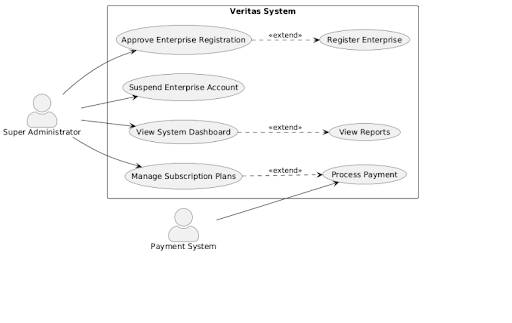
\includegraphics[height=0.75\textheight]{assets/uc_diagrams/uc_super_admin.png}
    \end{center}
\end{frame}

% =============================================================================
% Detailed Use Cases
% =============================================================================
\begin{frame}{UC-01: Approve Enterprise Registration}
    \begin{block}{Use Case Details}
        \begin{description}
            \item[Actor] Super Administrator
            \item[Precondition] Enterprise has submitted registration request
            \item[Postcondition] Enterprise account is approved and activated OR rejected with reason
        \end{description}
    \end{block}
    
    \begin{block}{Main Flow}
        \begin{enumerate}
            \item Super Admin logs into system dashboard
            \item System displays pending enterprise registration requests
            \item Super Admin reviews enterprise details (company info, contact, requested plan)
            \item Super Admin approves or rejects request
            \item If approved: System provisions tenant environment, generates credentials
            \item System sends notification email to enterprise
        \end{enumerate}
    \end{block}
\end{frame}

\begin{frame}{UC-08: Create Exam}
    \begin{center}
        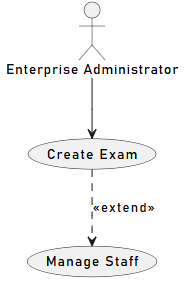
\includegraphics[width=0.7\textwidth]{assets/uc_diagrams/uc_create_exam.png}
    \end{center}
    
    \begin{block}{Key Features}
        \begin{itemize}
            \item Multi-step wizard for comprehensive exam configuration
            \item Question bank selection with targeted randomization
            \item Support for MCQ, True/False, Short Answer, Essay questions
            \item Configurable duration, passing score, negative marking
        \end{itemize}
    \end{block}
\end{frame}

\begin{frame}{UC-18: Start Exam (Candidate Flow)}
    \begin{center}
        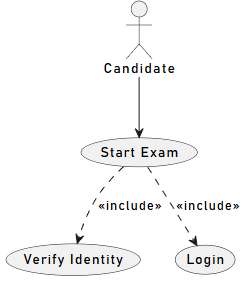
\includegraphics[width=0.65\textwidth]{assets/uc_diagrams/uc_start_exam.png}
    \end{center}
    
    \begin{block}{Critical Steps}
        \begin{enumerate}
            \item Candidate authenticates with enterprise token/ID
            \item System verifies exam schedule and candidate eligibility
            \item Candidate completes identity verification (facial capture)
            \item System performs system check (camera, browser compatibility)
            \item Exam interface loads in fullscreen mode with proctoring active
        \end{enumerate}
    \end{block}
\end{frame}

% =============================================================================
% Sequence Diagrams
% =============================================================================
\begin{frame}{Sequence Diagrams: Overview}
    \textbf{Sequence diagrams illustrate interactions between actors and system for key use cases}
    
    \begin{block}{Categories Covered}
        \begin{enumerate}
            \item \textbf{Enterprise Onboarding \& Lifecycle}
            \begin{itemize}
                \item Enterprise Registration \& Approval Workflow
                \item Subscription Payment \& Dunning Process
            \end{itemize}
            
            \item \textbf{Authentication \& Security}
            \begin{itemize}
                \item Candidate Login with Face Verification
                \item Session Timeout \& Re-authentication
            \end{itemize}
            
            \item \textbf{Examination Management}
            \begin{itemize}
                \item Bulk Enrollment \& Token Generation
                \item Exam Configuration (Targeted Randomization)
            \end{itemize}
        \end{enumerate}
    \end{block}
\end{frame}

\begin{frame}{Sequence Diagrams: Overview (continued)}
    \begin{block}{Categories Covered (continued)}
        \begin{enumerate}
            \setcounter{enumi}{3}
            \item \textbf{Candidate Exam Experience}
            \begin{itemize}
                \item Answer Auto-Save \& Sync
            \end{itemize}
            
            \item \textbf{AI Proctoring \& Monitoring}
            \begin{itemize}
                \item Proctoring Event Loop
            \end{itemize}
            
            \item \textbf{Grading \& Reporting}
            \begin{itemize}
                \item Hybrid Grading Workflow
                \item Async Report Generation
            \end{itemize}
        \end{enumerate}
    \end{block}
    
    \vspace{0.3cm}
    \textit{Each diagram maps to specific functional requirements}
\end{frame}

\begin{frame}{SD: Enterprise Registration \& Approval}
    \begin{center}
        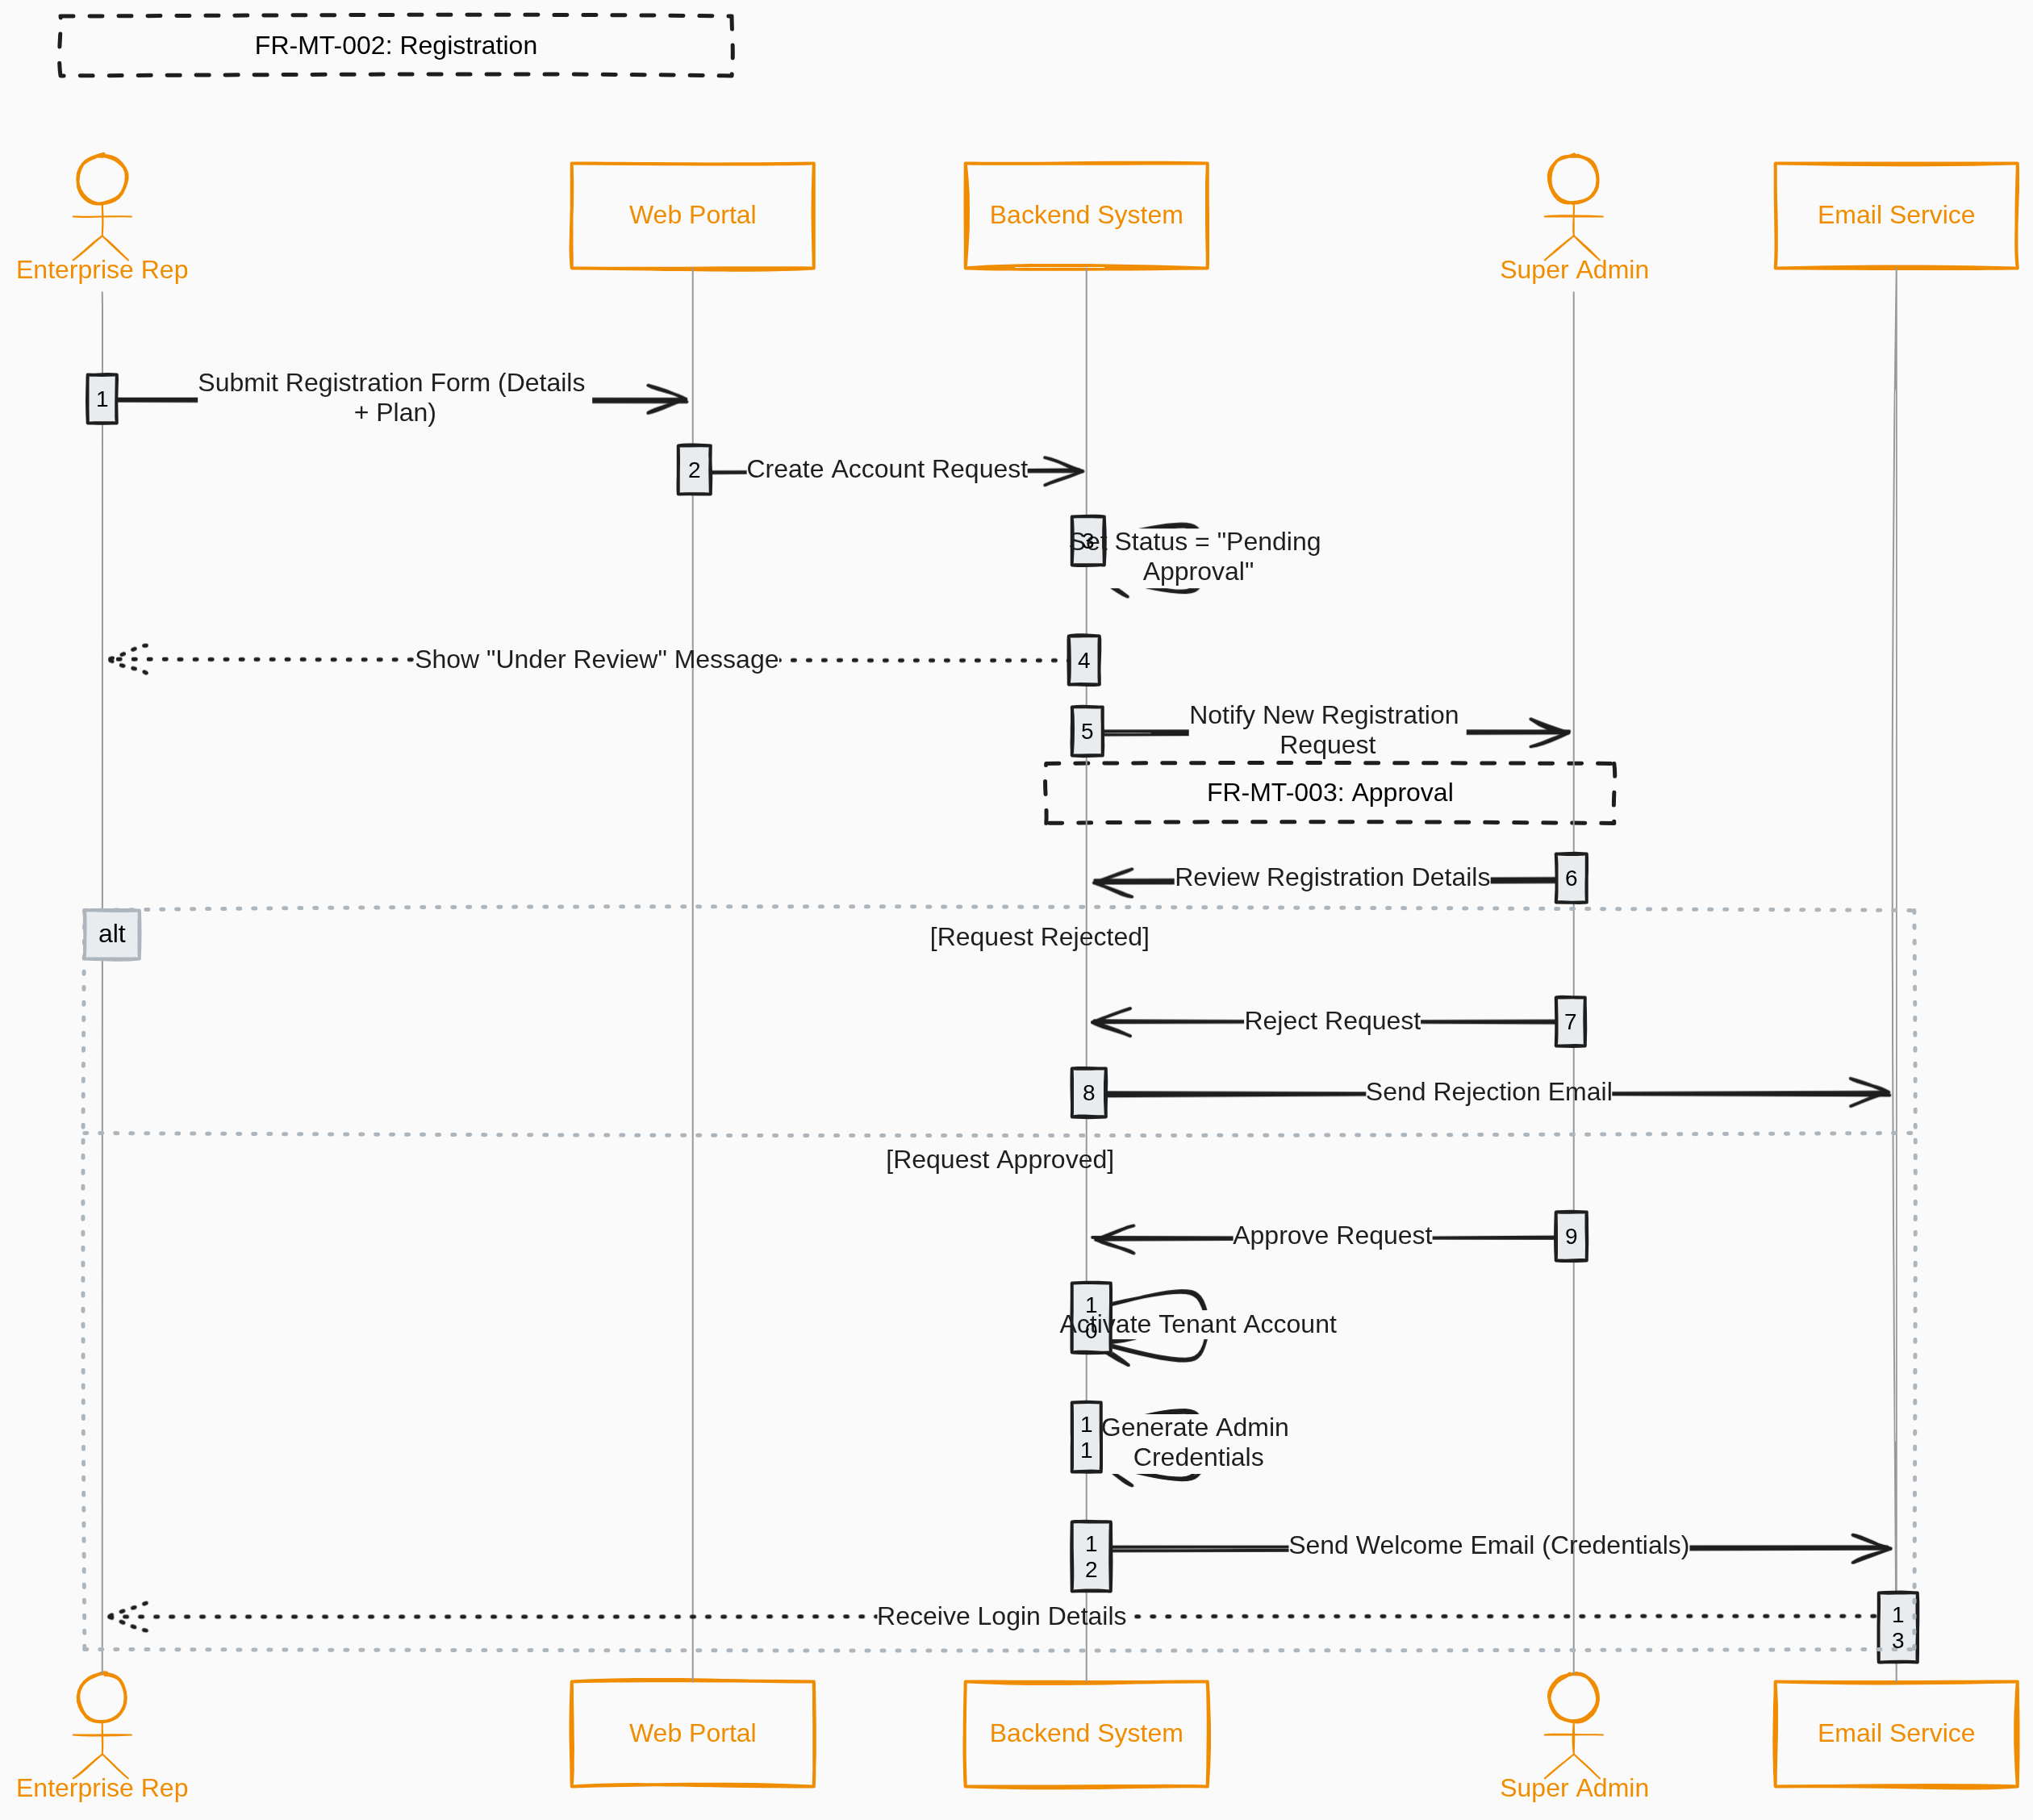
\includegraphics[width=0.9\textwidth]{assets/seq_diagrams/Enterprise Registration.png}
    \end{center}
    
    \textbf{Implements:} FR-MT-002, FR-MT-003
\end{frame}

\begin{frame}{SD: Subscription Payment \& Dunning}
    \begin{center}
        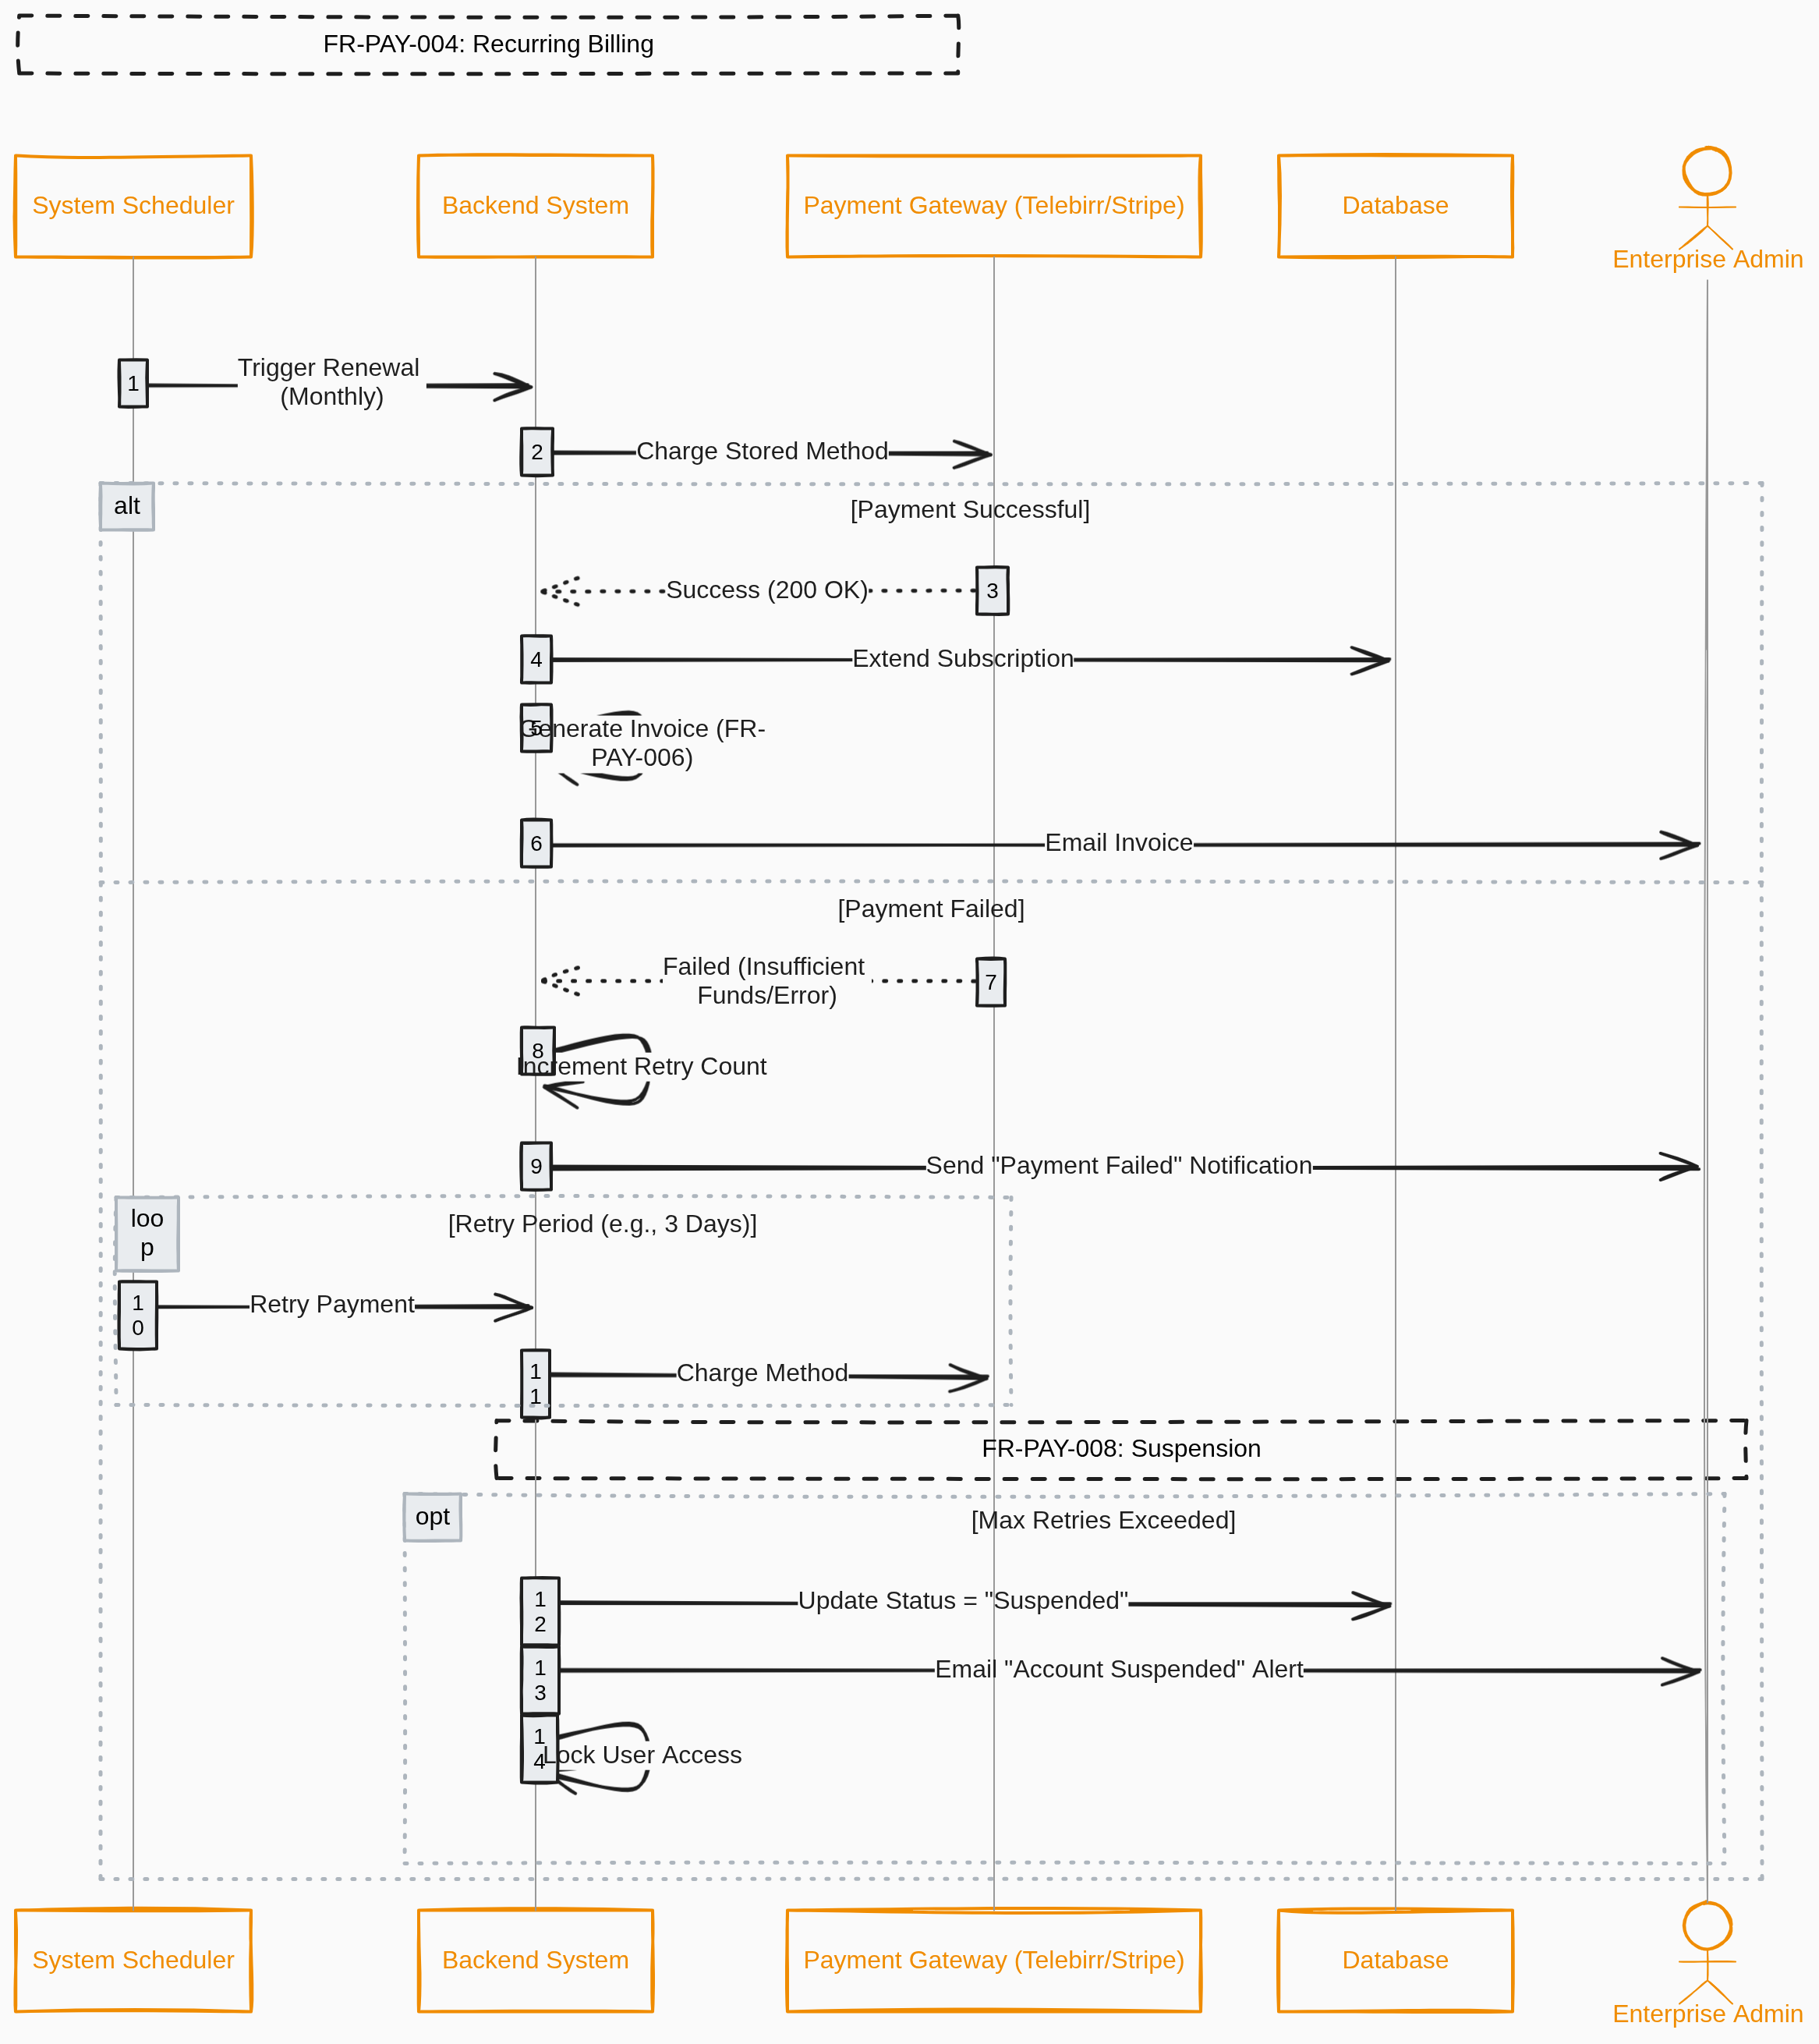
\includegraphics[width=0.9\textwidth]{assets/seq_diagrams/Subscription Payment & Dunning (Suspension).png}
    \end{center}
    
    \textbf{Implements:} FR-PAY-004, FR-PAY-008 \\
    \textit{Financial lifecycle: billing, retry loop, account suspension}
\end{frame}

\begin{frame}{SD: Candidate Login with Face Verification}
    \begin{center}
        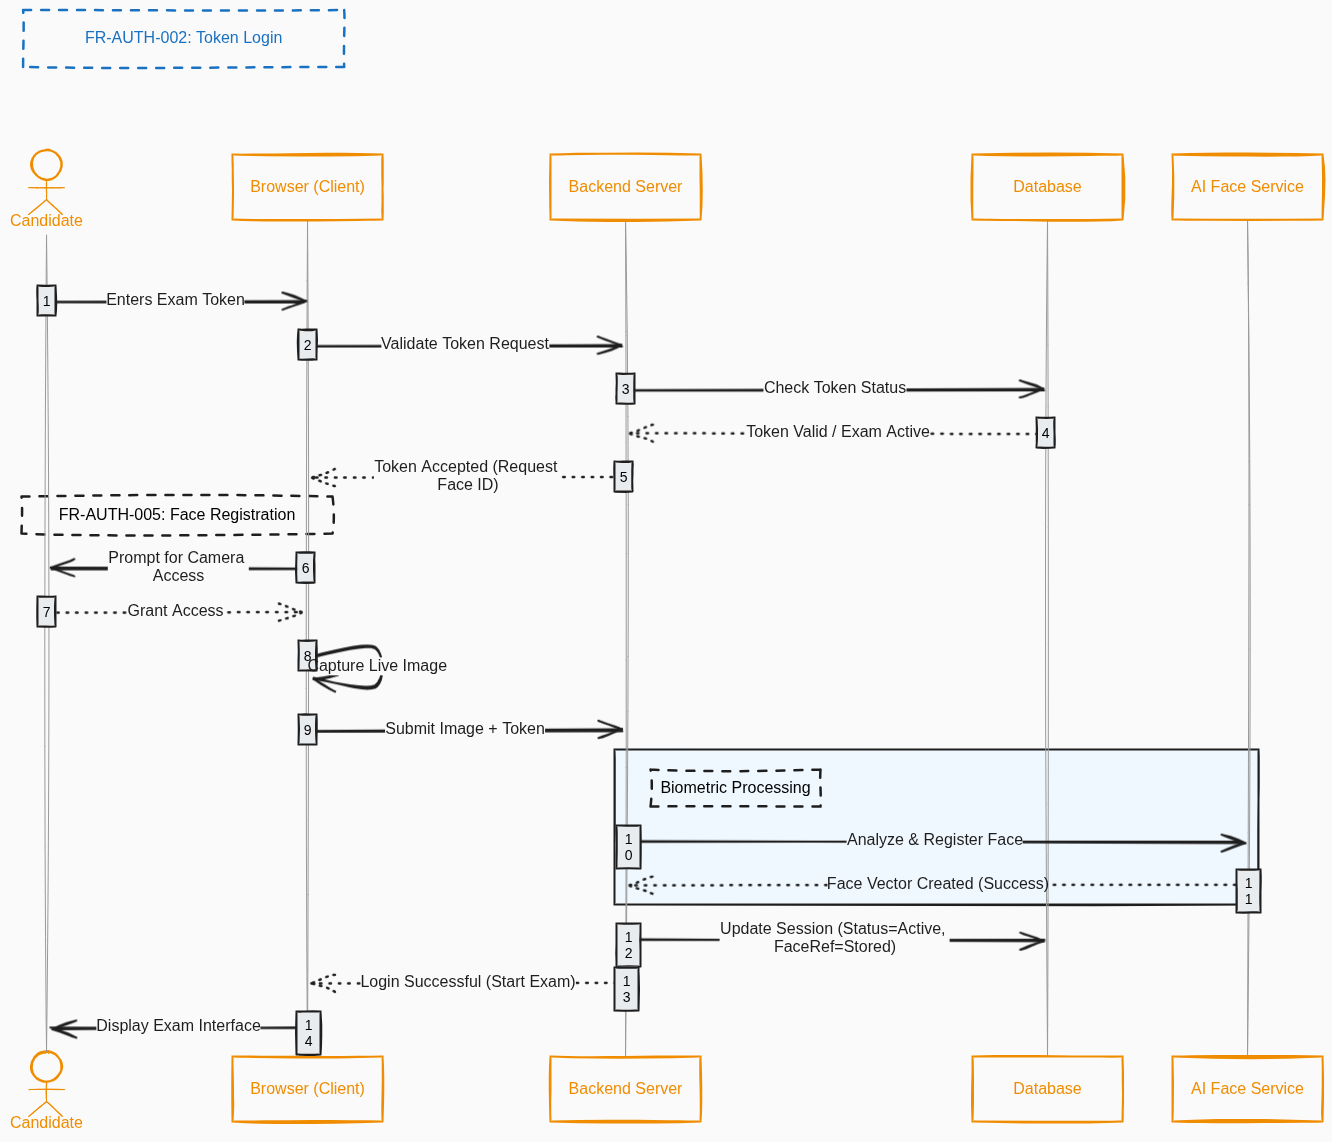
\includegraphics[width=0.9\textwidth]{assets/seq_diagrams/FR-2.png}
    \end{center}
    
    \textbf{Implements:} FR-AUTH-002, FR-AUTH-005 \\
    \textit{Multi-factor authentication to eliminate impersonation}
\end{frame}

\begin{frame}{SD: Session Timeout \& Re-authentication}
    \begin{center}
        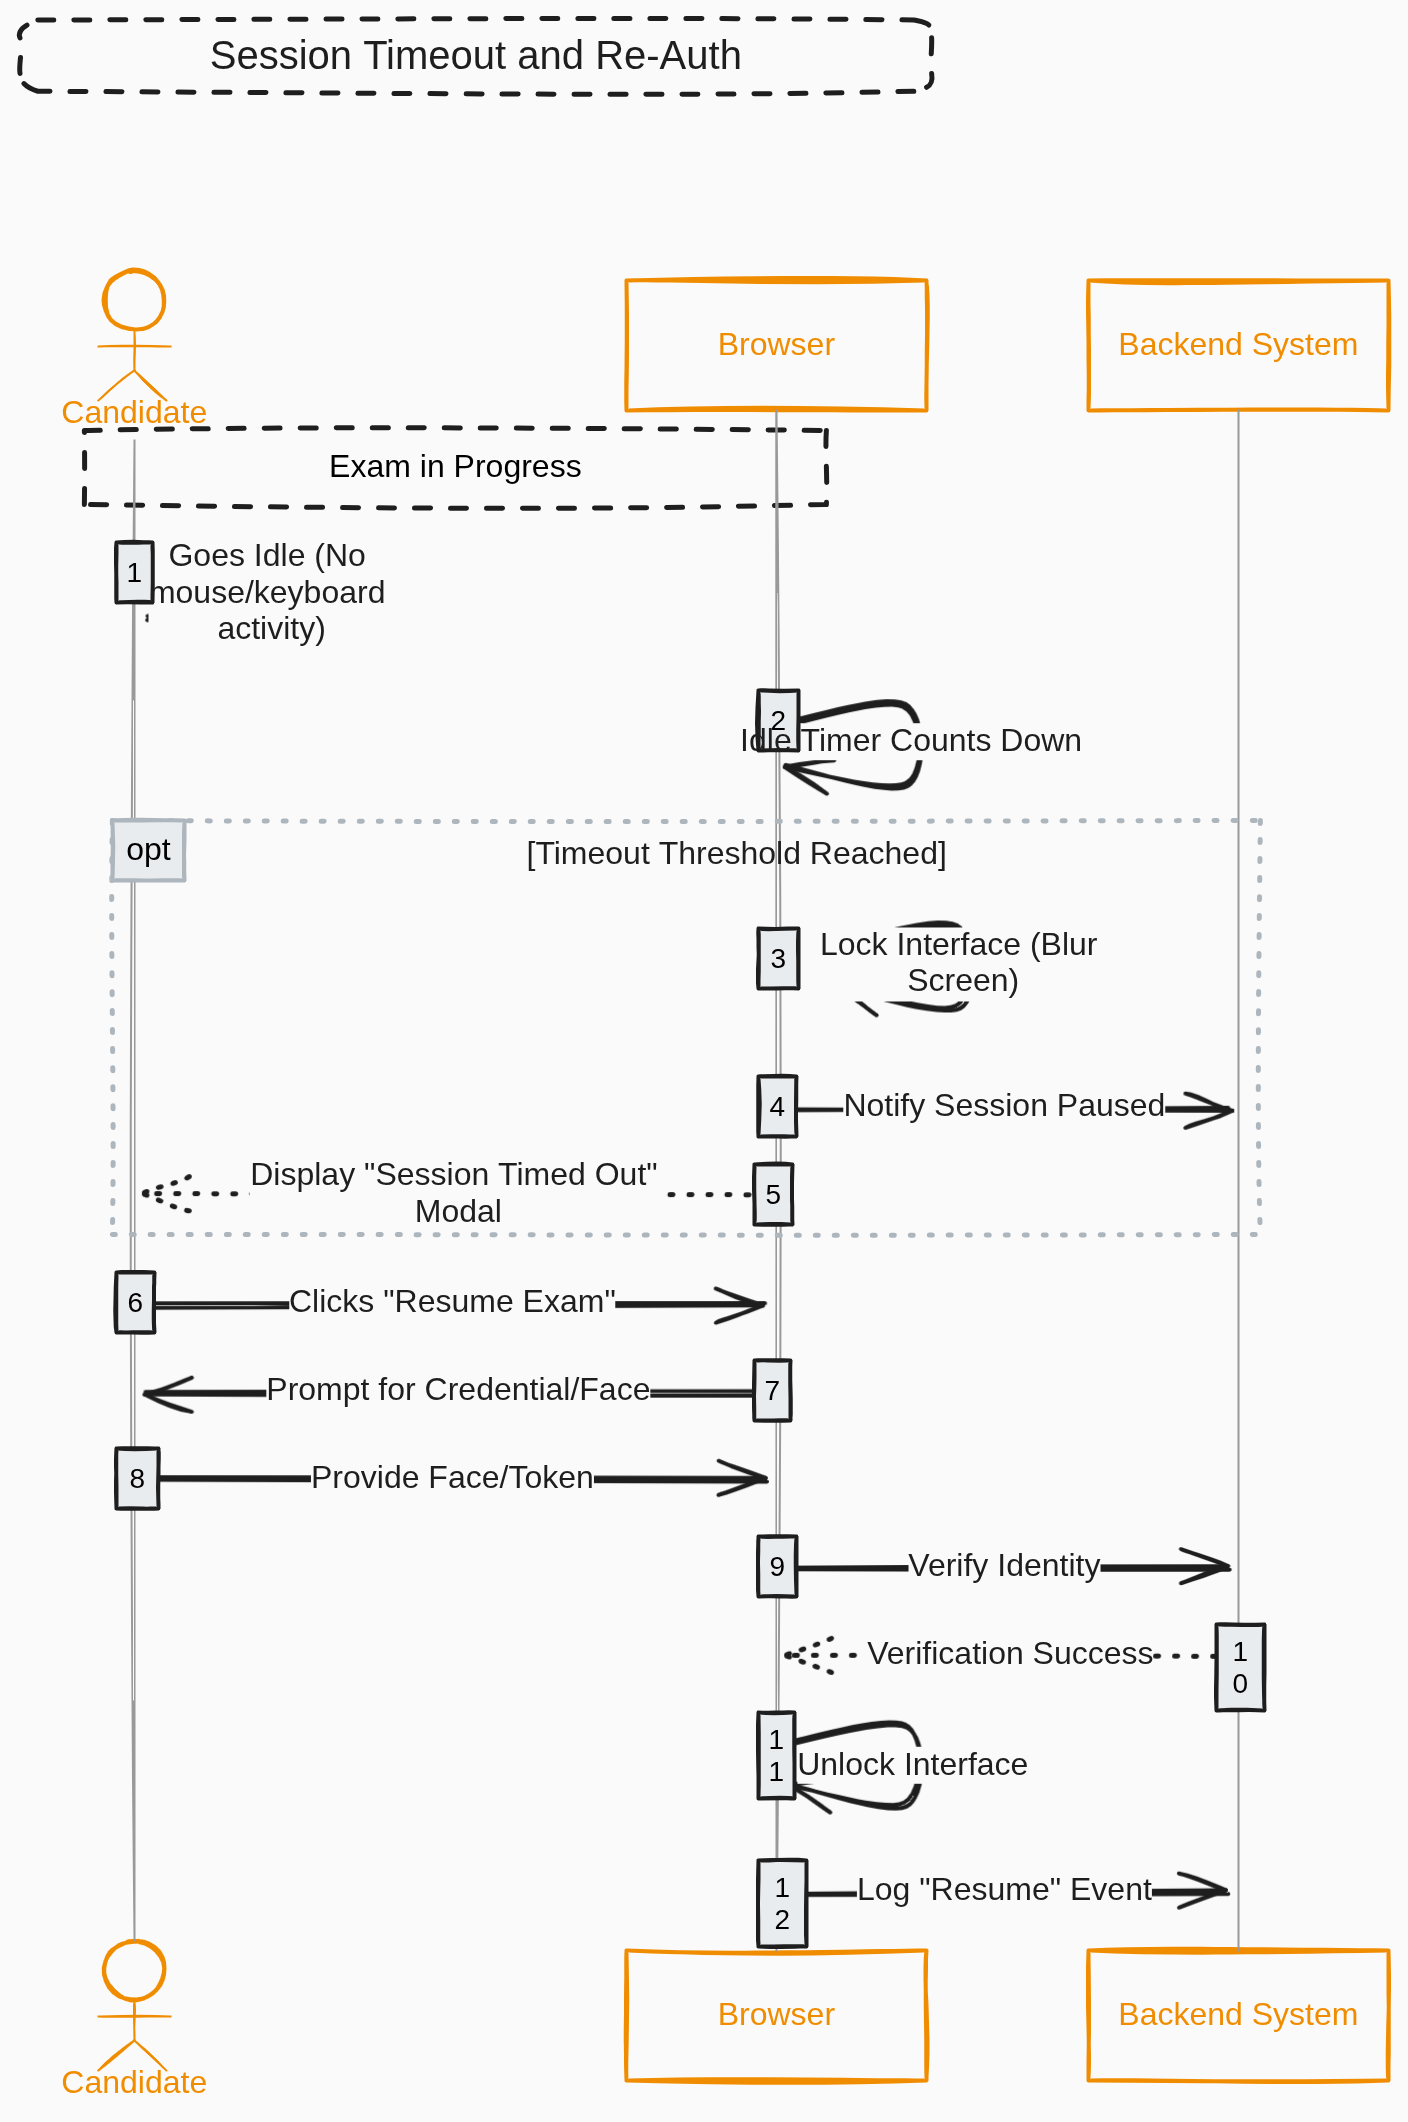
\includegraphics[width=0.75\textwidth]{assets/seq_diagrams/Session Timeout and Re-Auth.png}
    \end{center}
    
    \textbf{Implements:} FR-AUTH-007 \\
    \textit{Security response to user inactivity - prevents exploitation of unattended workstation}
\end{frame}

\begin{frame}{SD: Bulk Enrollment \& Token Generation}
    \begin{center}
        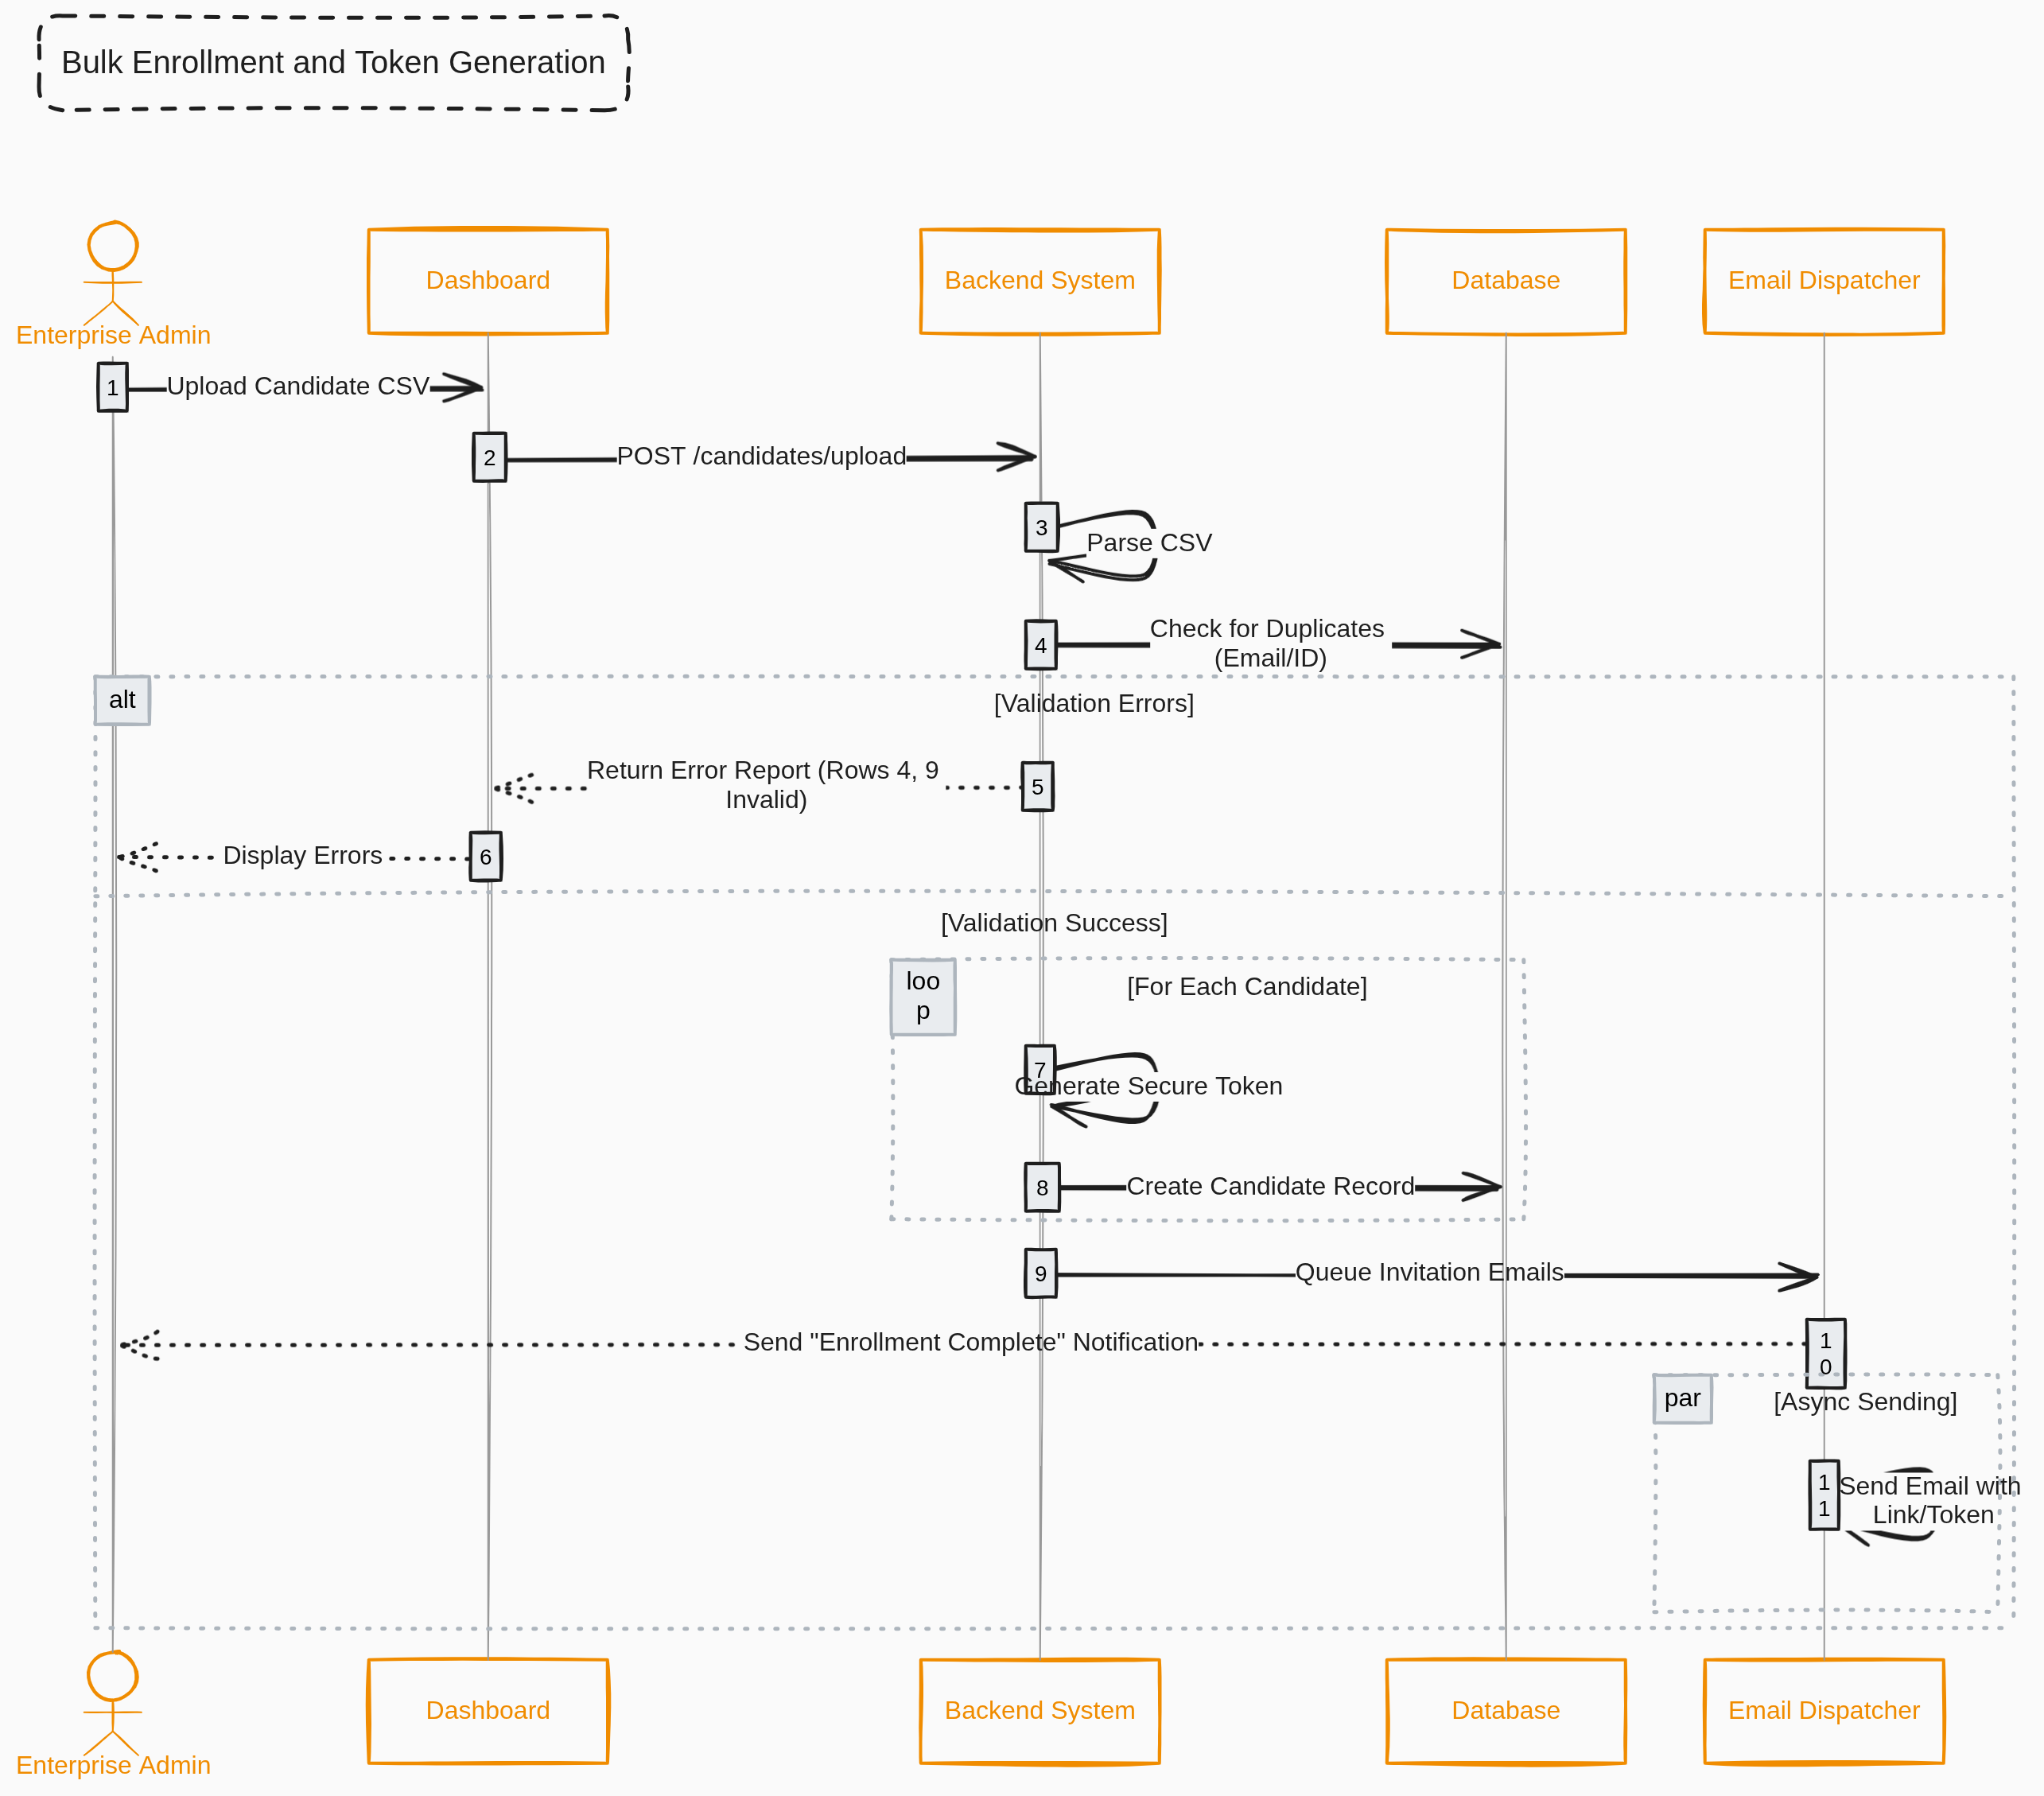
\includegraphics[width=0.9\textwidth]{assets/seq_diagrams/Bulk Enrollment and Token Gen.png}
    \end{center}
    
    \textbf{Implements:} FR-EXM-004 \\
    \textit{High-volume data processing for large exams: CSV upload, validation, token generation, email dispatch}
\end{frame}

\begin{frame}{SD: Exam Configuration (Targeted Randomization)}
    \begin{center}
        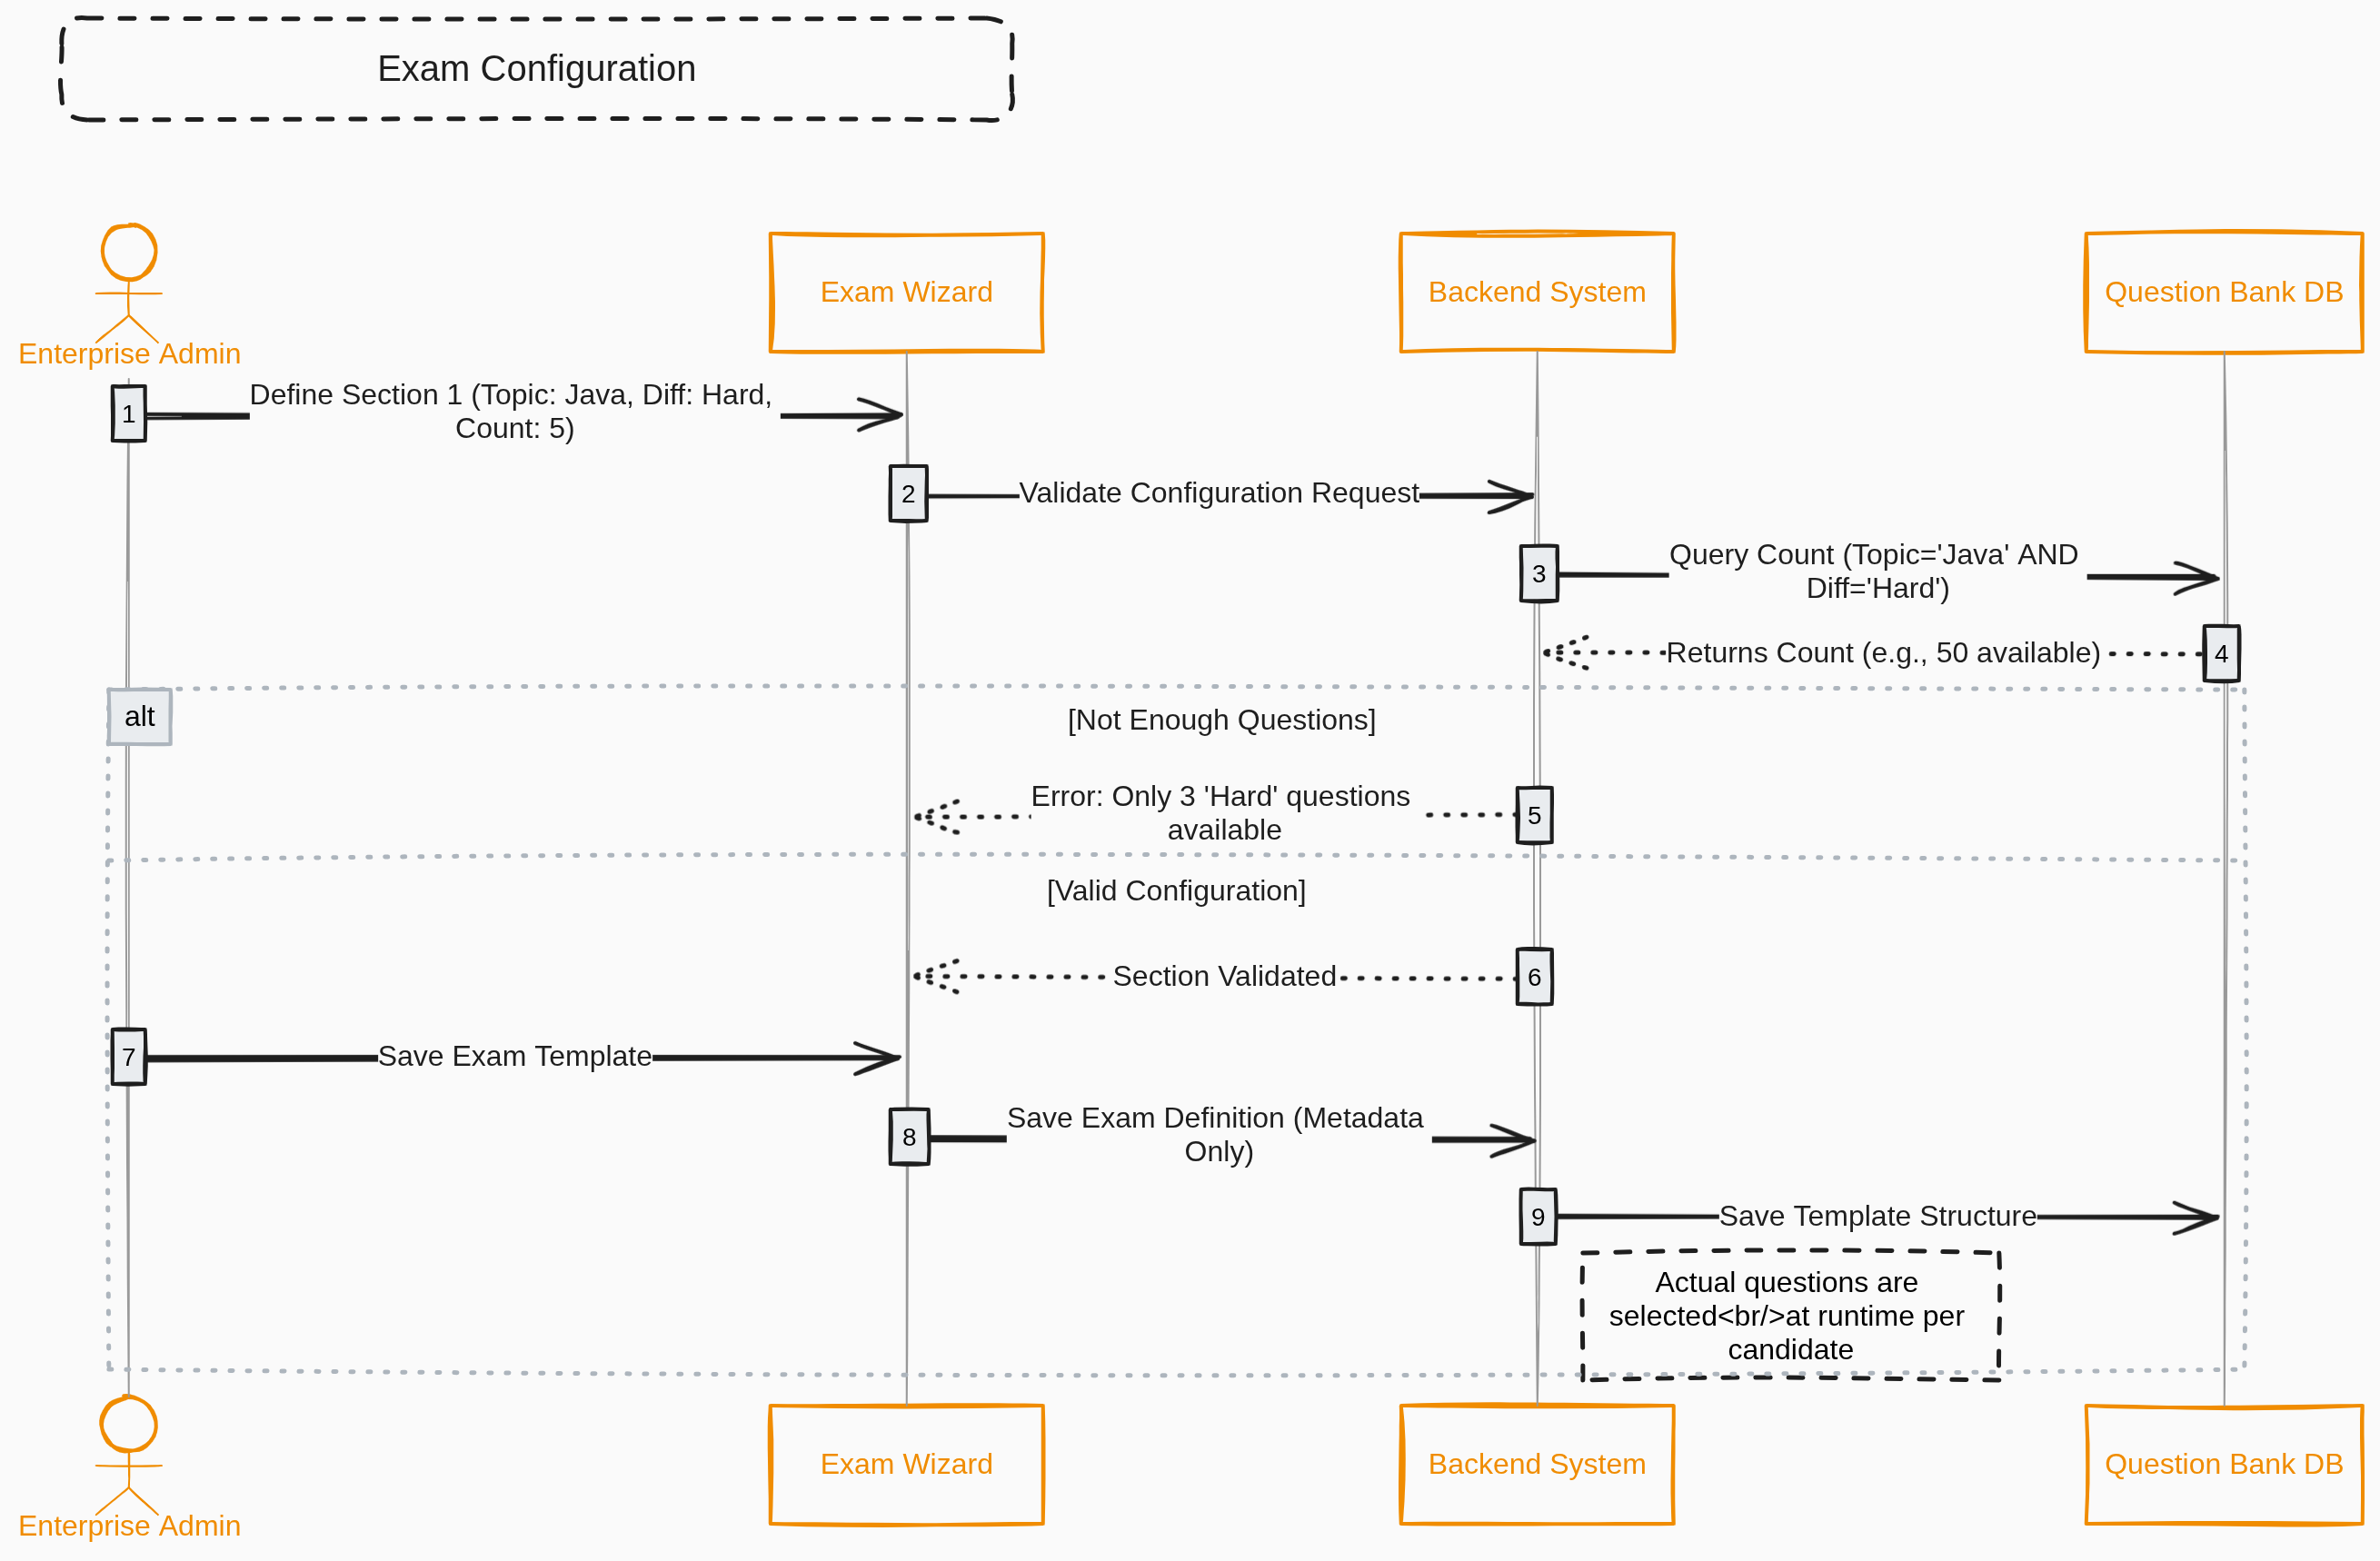
\includegraphics[width=0.9\textwidth]{assets/seq_diagrams/Exam Configuration.png}
    \end{center}
    
    \textbf{Implements:} FR-EXM-002 \\
    \textit{Dynamic, randomized exams: Admin defines criteria, system validates question bank, saves template}
\end{frame}

\begin{frame}{SD: Answer Auto-Save \& Sync}
    \begin{center}
        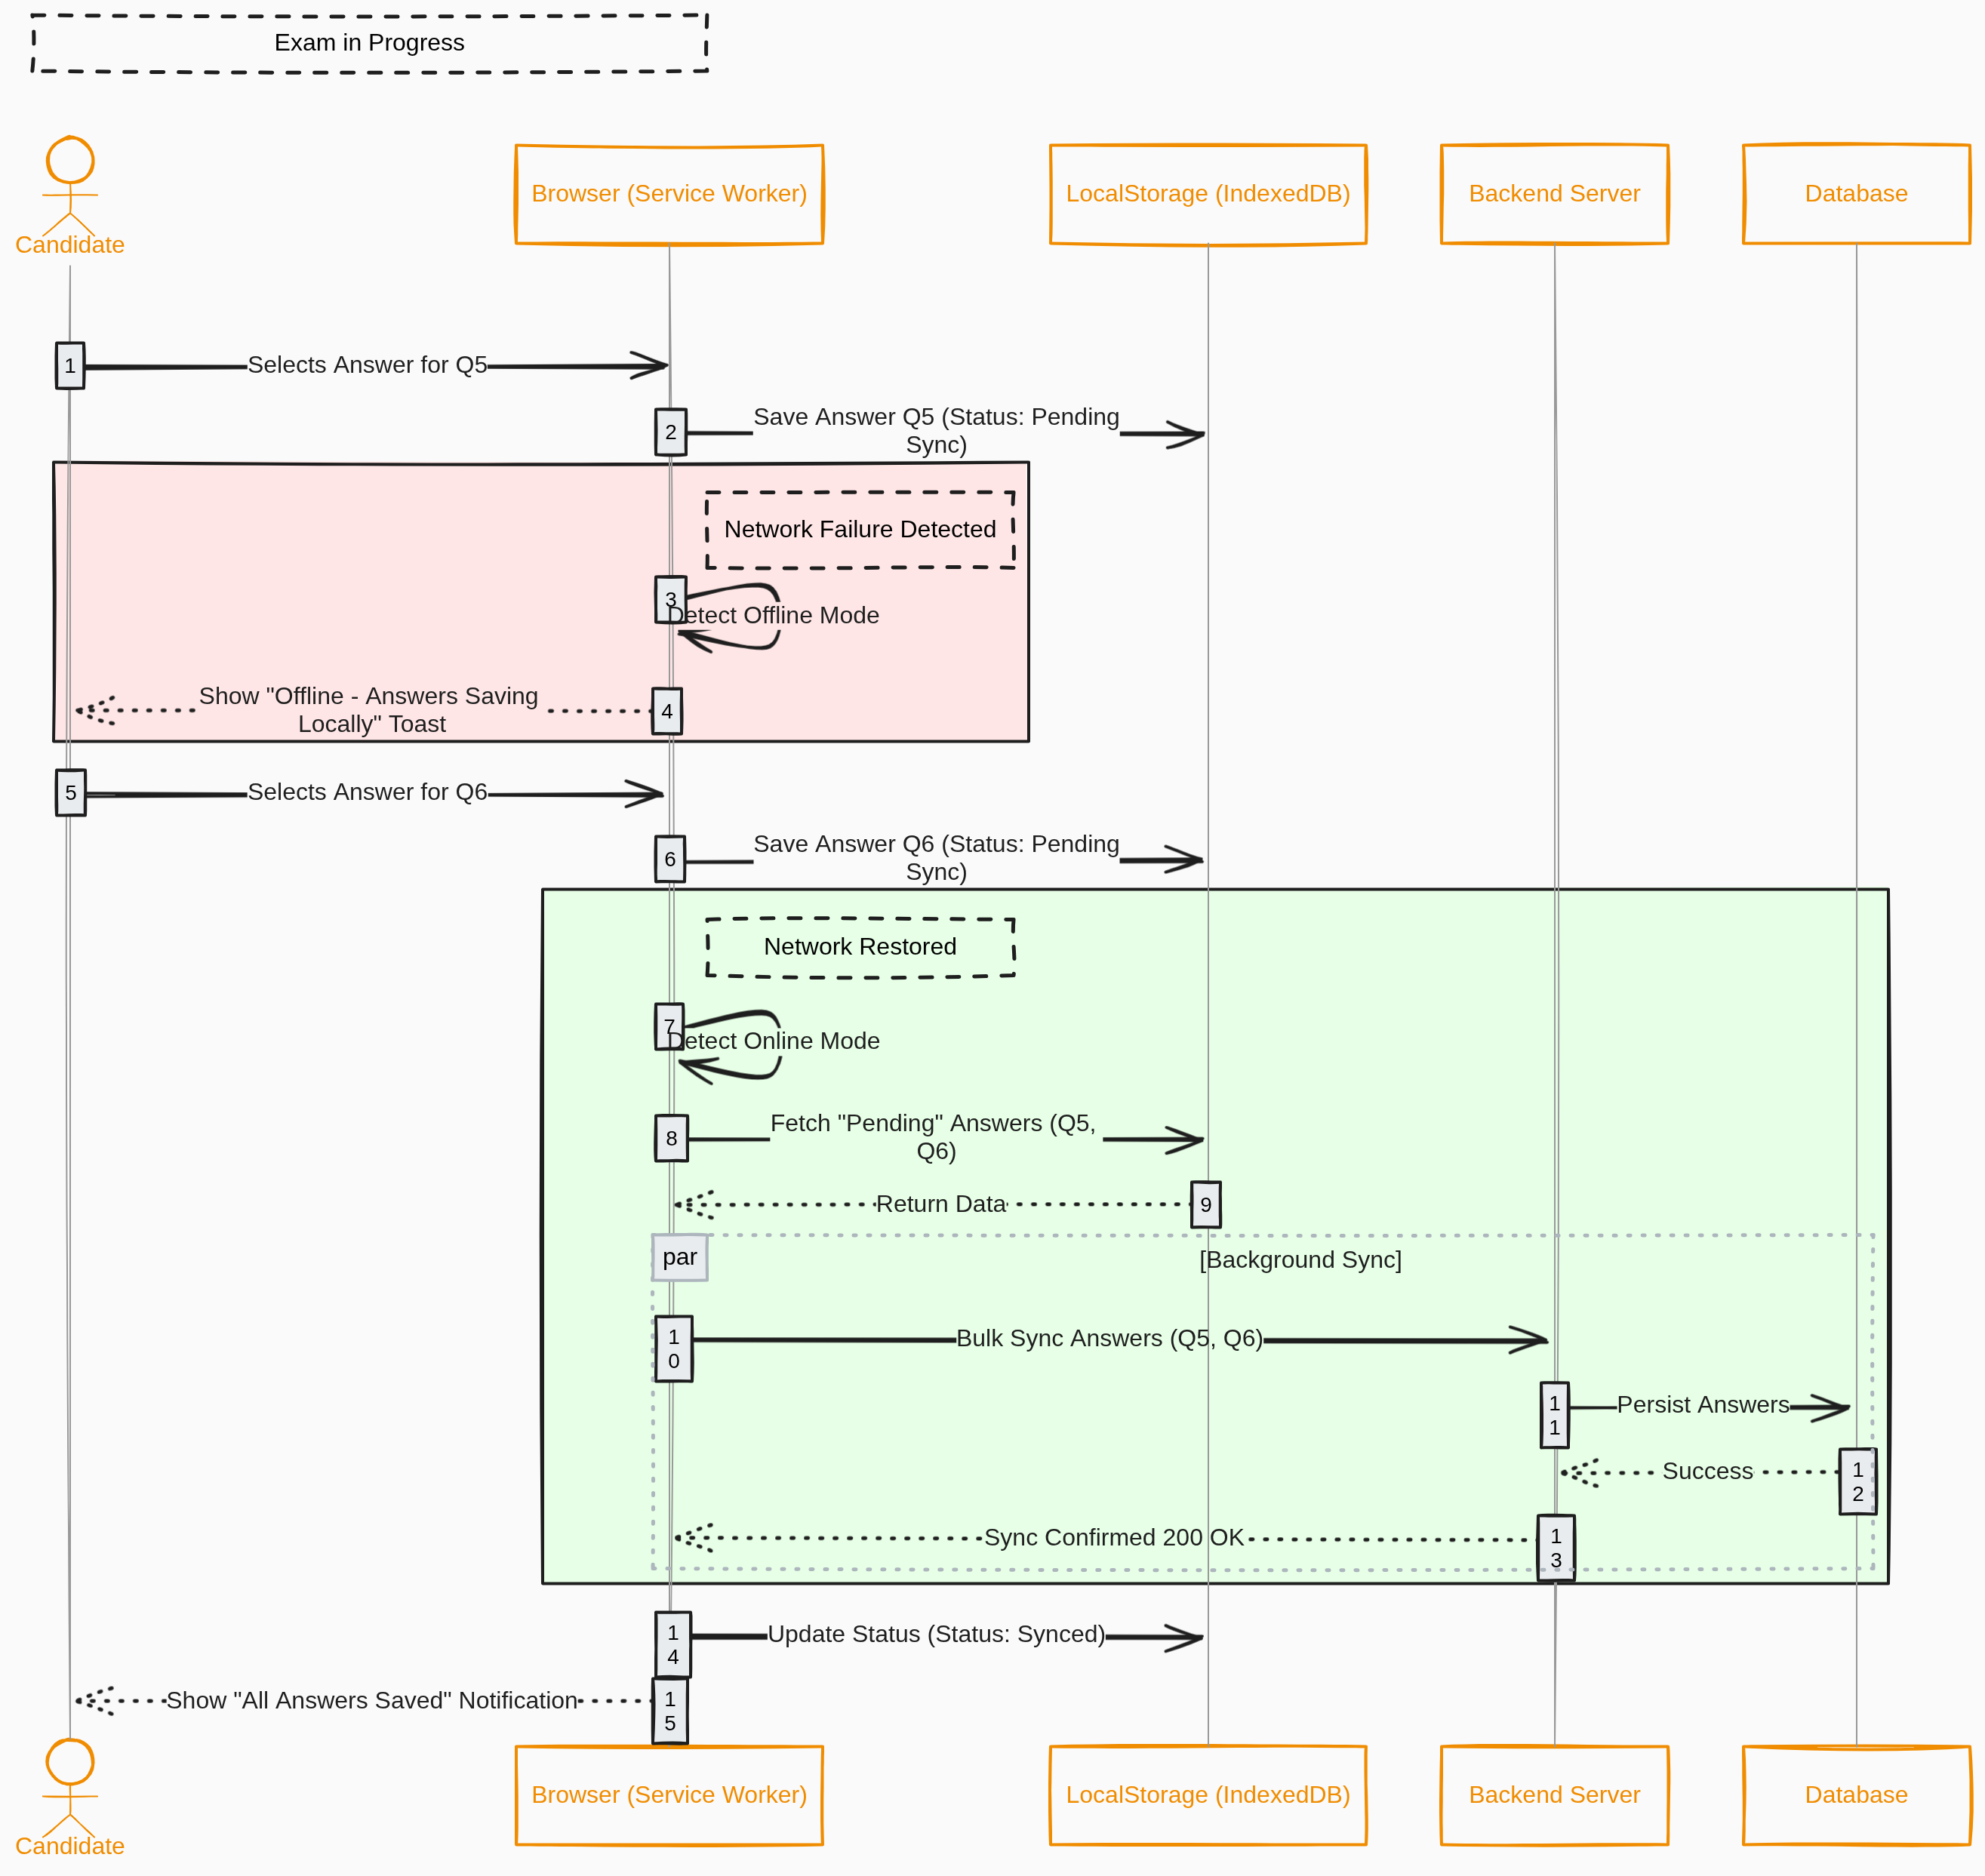
\includegraphics[width=0.9\textwidth]{assets/seq_diagrams/Exam in Progress.png}
    \end{center}
    
    \textbf{Implements:} FR-CAND-004 \\
    \textit{Data synchronization protecting candidate progress: local storage + periodic server sync}
\end{frame}

\begin{frame}{SD: Proctoring Event Loop}
    \begin{center}
        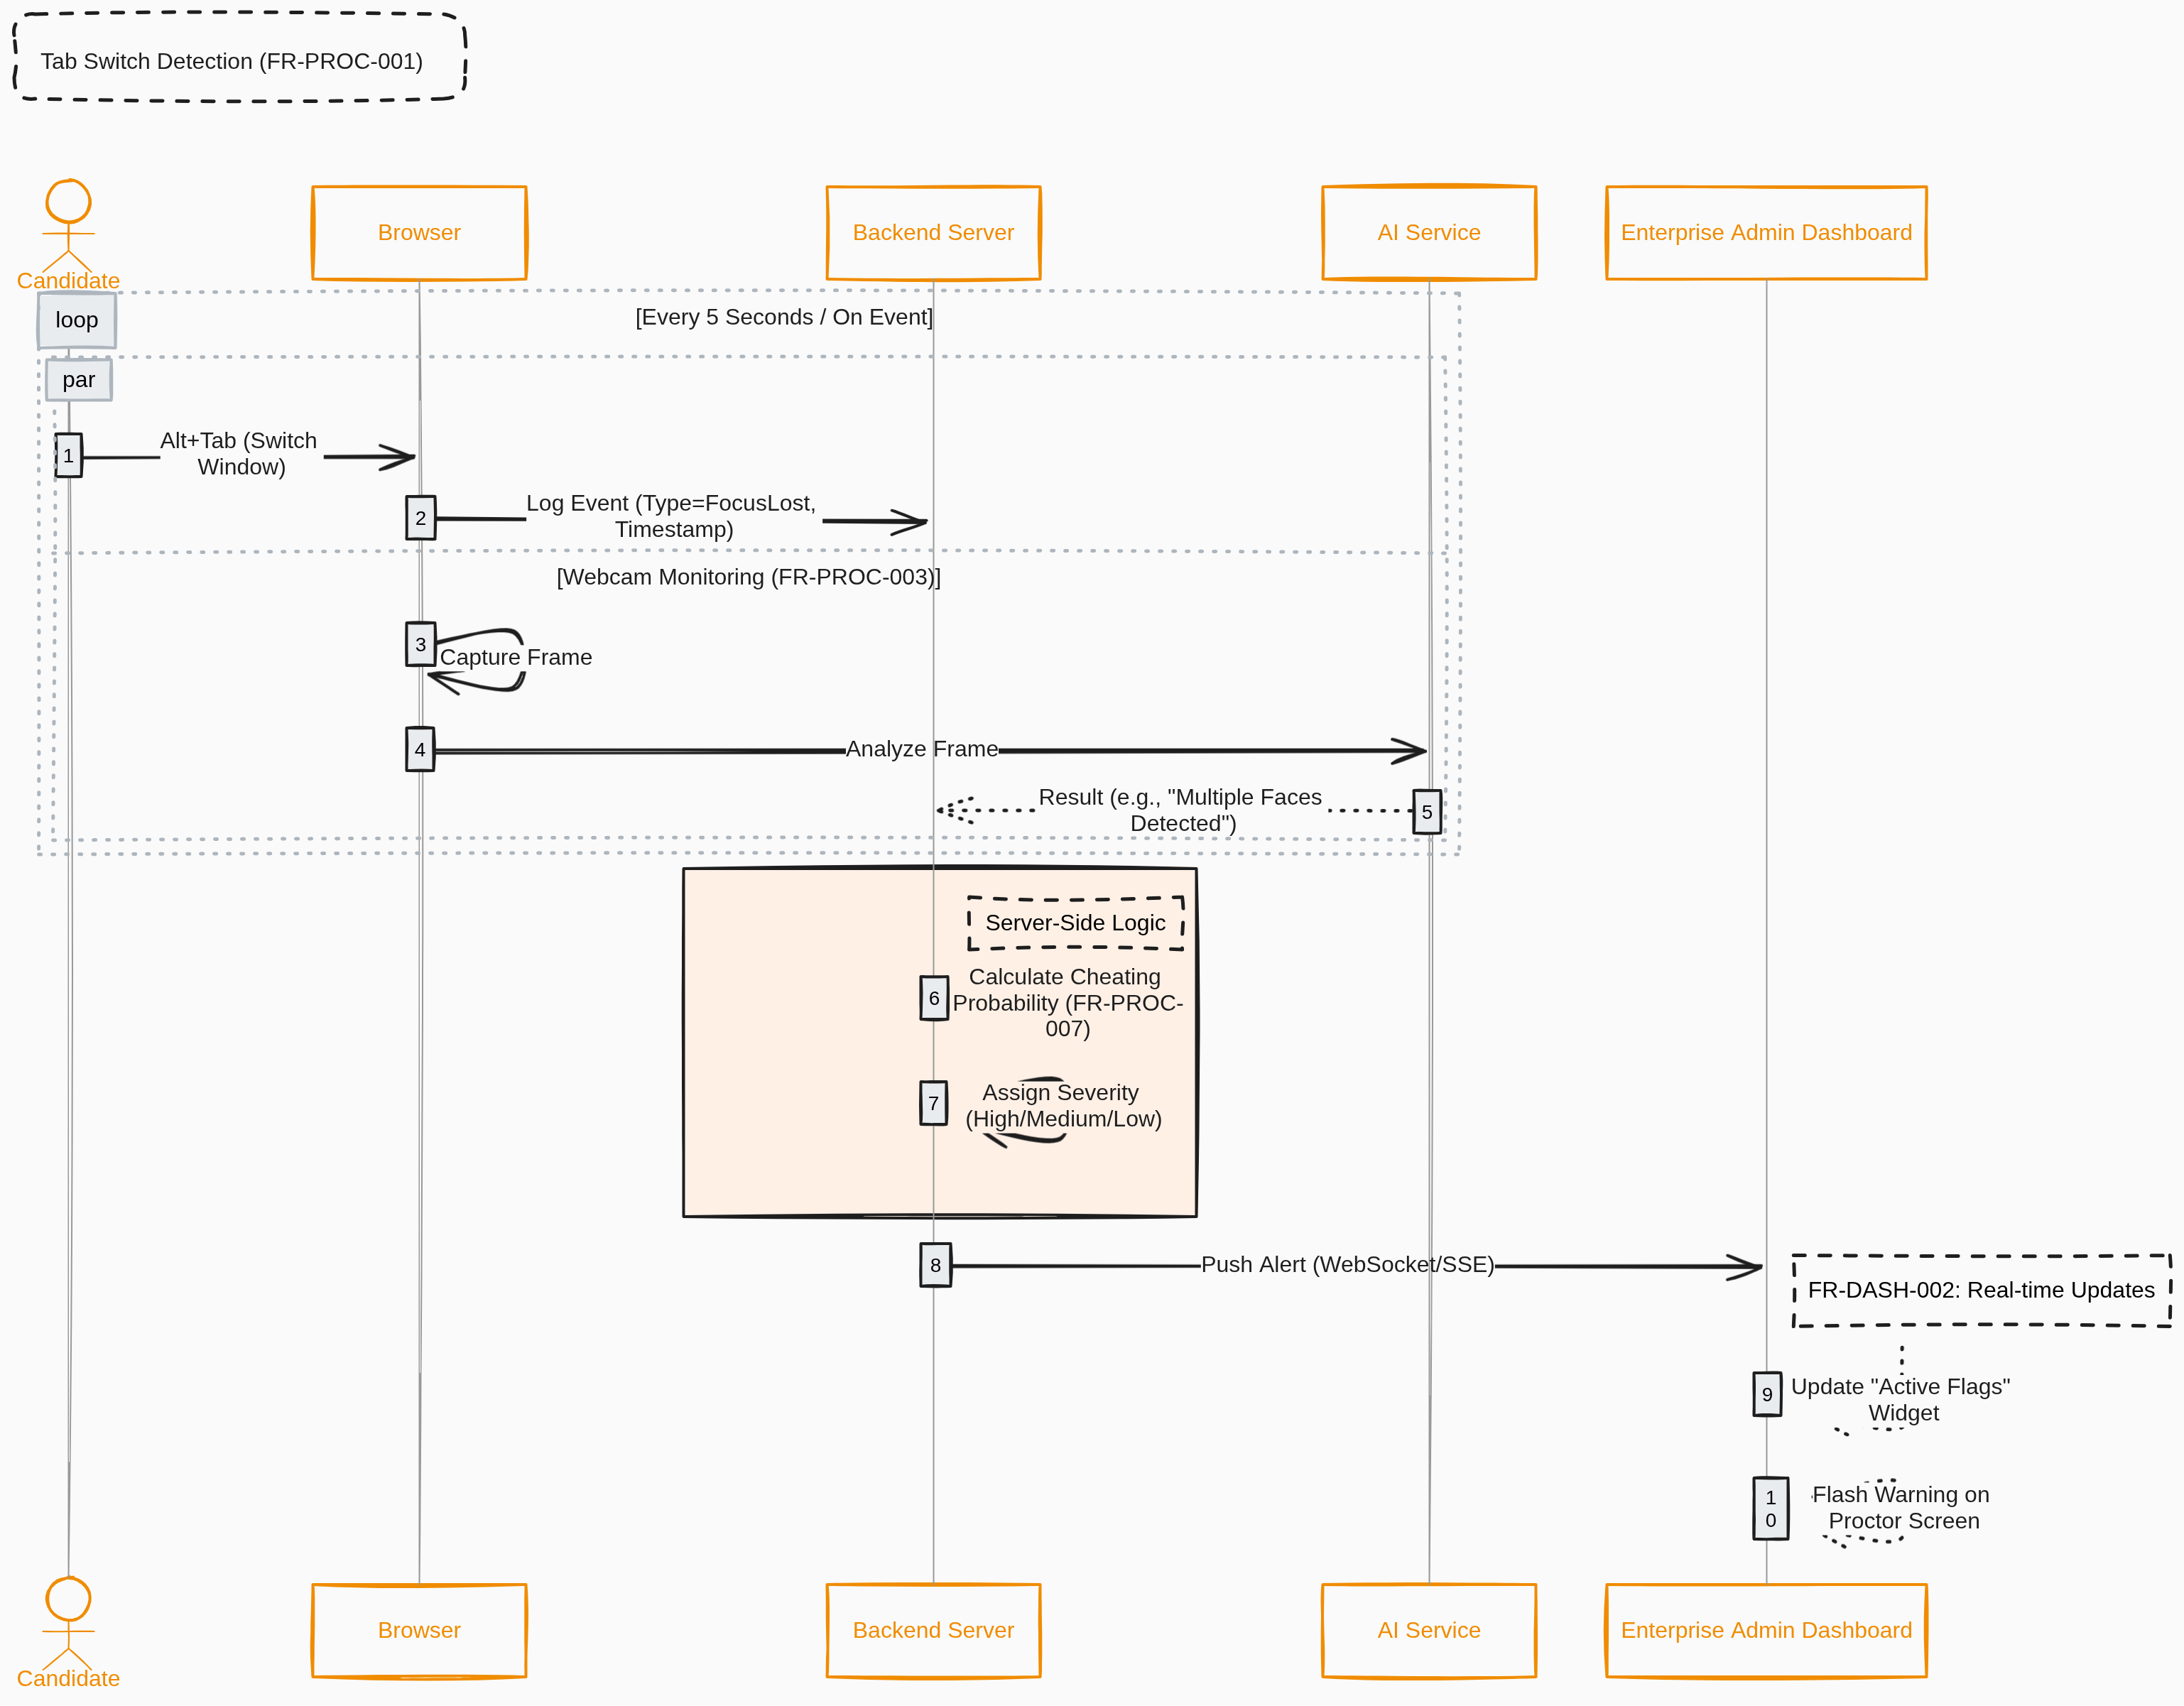
\includegraphics[width=0.9\textwidth]{assets/seq_diagrams/Tab Switch Detection.png}
    \end{center}
    
    \textbf{Implements:} FR-PROC-001, FR-DASH-002 \\
    \textit{Real-time monitoring: browser events + webcam AI analysis → cheating probability score → Admin dashboard}
\end{frame}

\begin{frame}{SD: Hybrid Grading Workflow}
    \begin{center}
        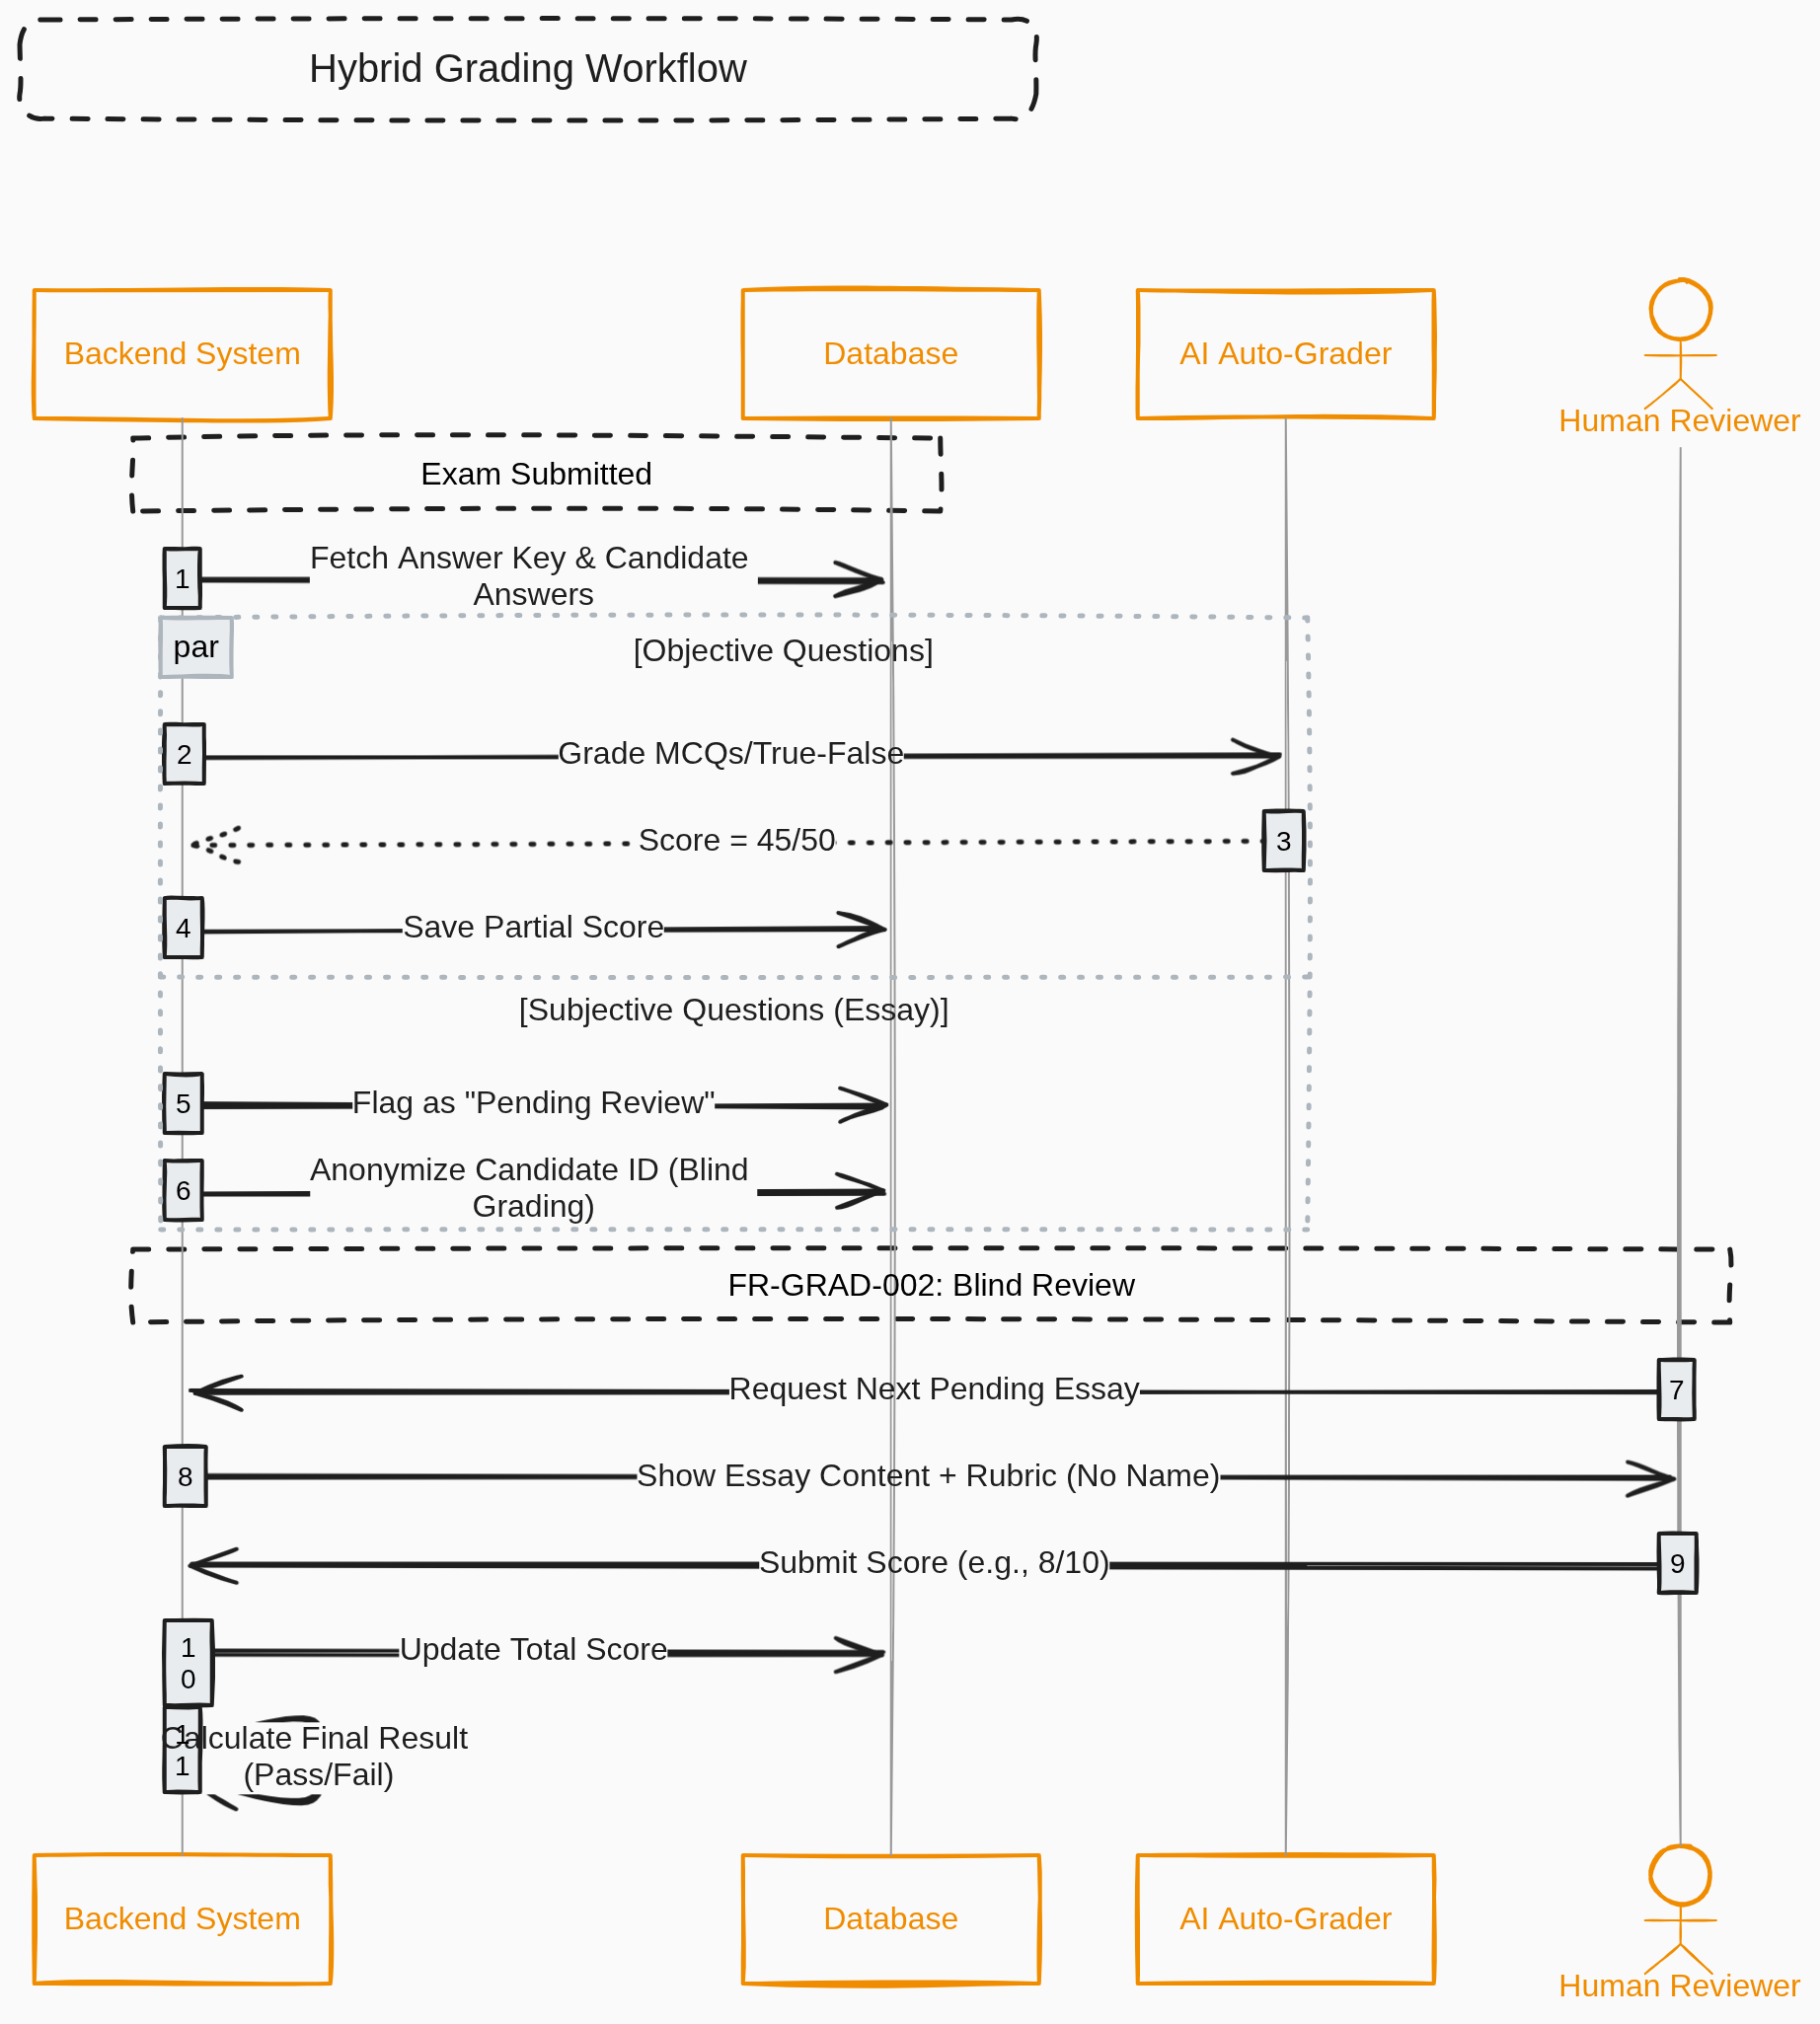
\includegraphics[width=0.9\textwidth]{assets/seq_diagrams/Hybrid Grading Workflow.png}
    \end{center}
    
    \textbf{Implements:} FR-GRAD-001, FR-GRAD-002 \\
    \textit{Split processing: Objective (auto-graded) + Subjective (blind human review)}
\end{frame}

\begin{frame}{SD: Async Report Generation}
    \begin{center}
        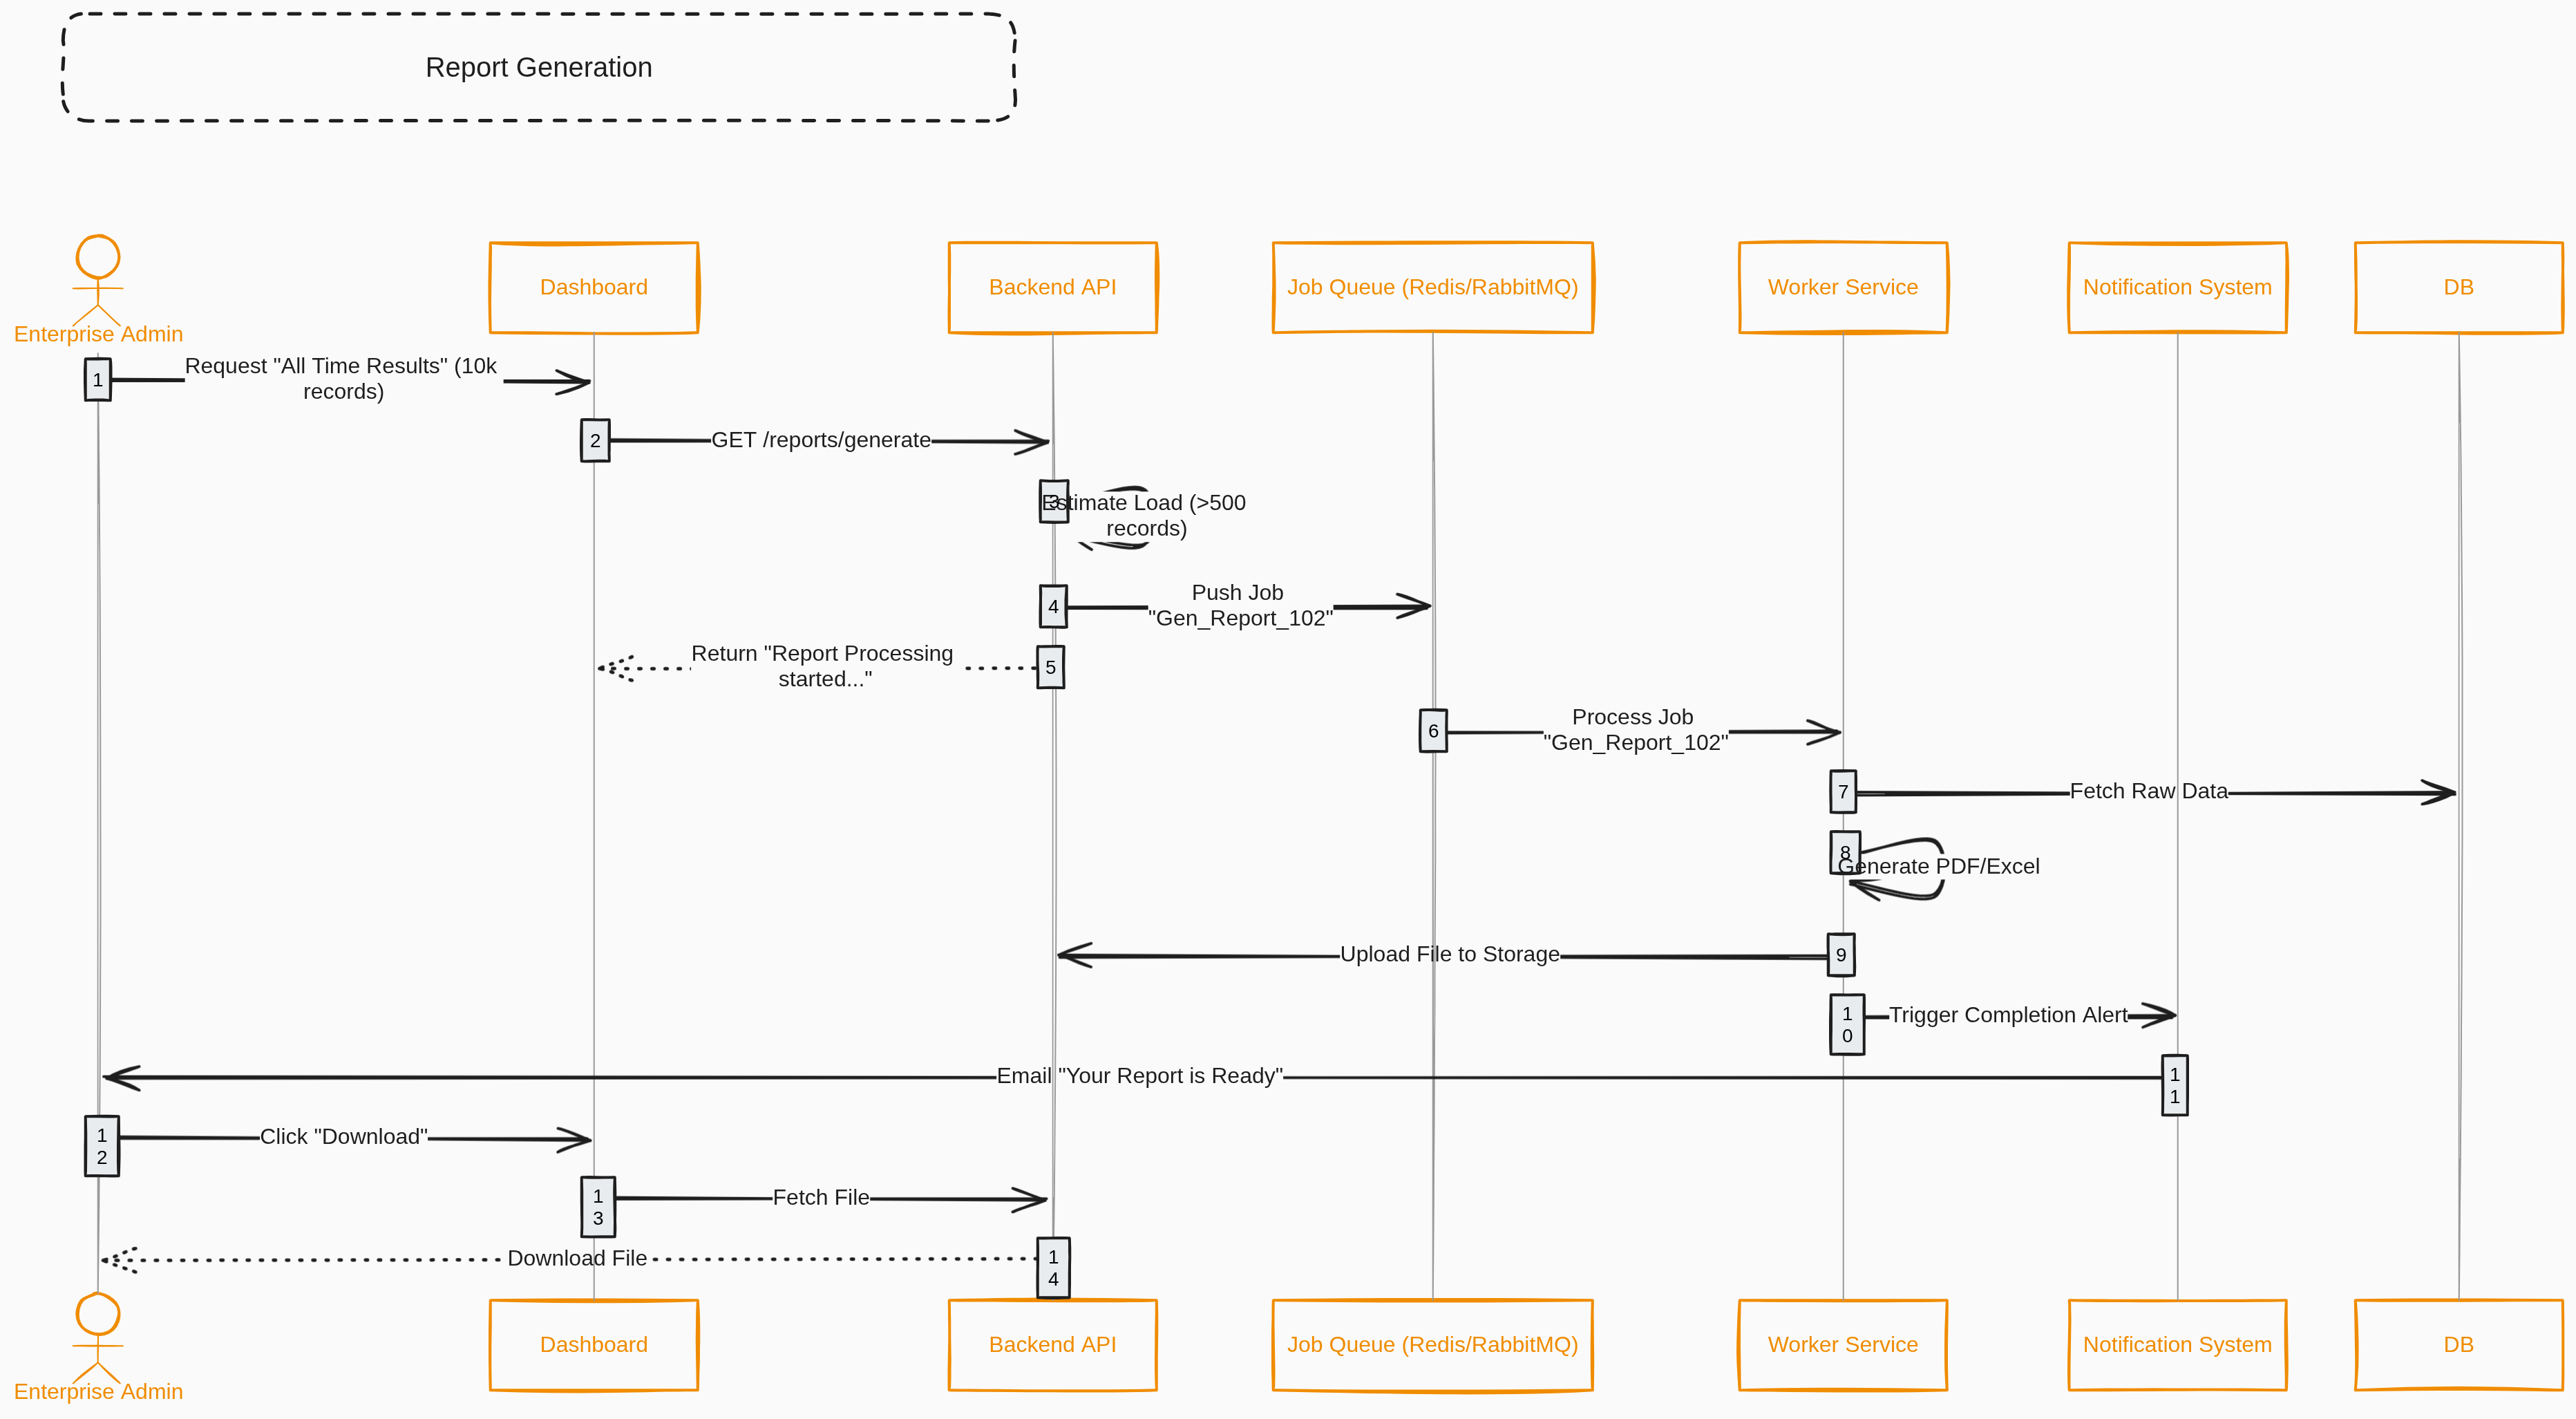
\includegraphics[width=0.9\textwidth]{assets/seq_diagrams/Report Generation.png}
    \end{center}
    
    \textbf{Implements:} FR-DASH-003 \\
    \textit{Performance optimization: Large reports ($\geq$500 records) offloaded to job queue, background processing}
\end{frame}

% =============================================================================
% Activity Diagrams
% =============================================================================
\begin{frame}{Activity Diagrams: Overview}
    \textbf{Activity diagrams model workflows, decision points, and parallel activities}
    
    \begin{block}{Four Main Workflows}
        \begin{enumerate}
            \item \textbf{Enterprise Registration \& Authentication}
            \begin{itemize}
                \item Organization registration → admin approval → subscription selection → payment → dashboard access
            \end{itemize}
            
            \item \textbf{Exam Creation \& Scheduling}
            \begin{itemize}
                \item Admin login → exam config (questions, duration, scoring, randomization) → candidate assignment → publish
            \end{itemize}
            
            \item \textbf{Candidate Exam + AI Proctoring}
            \begin{itemize}
                \item Candidate login → identity verification (facial) → exam with continuous AI monitoring → submission
            \end{itemize}
            
            \item \textbf{Grading + Certificate Generation}
            \begin{itemize}
                \item Submission received → auto-grade objective + manual blind-grade subjective → calculate score → analyze proctoring → certificate or flag
            \end{itemize}
        \end{enumerate}
    \end{block}
\end{frame}

\begin{frame}{AD: Enterprise Registration \& Authentication}
    \begin{center}
        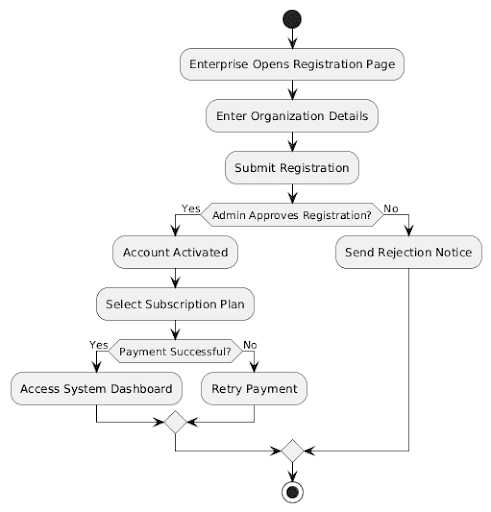
\includegraphics[width=0.9\textwidth]{assets/activity_diagrams/Enterprise Registration and Authentication.png}
    \end{center}
    
    \textit{Controlled system access with subscription enforcement}
\end{frame}

\begin{frame}{AD: Exam Creation \& Scheduling}
    \begin{center}
        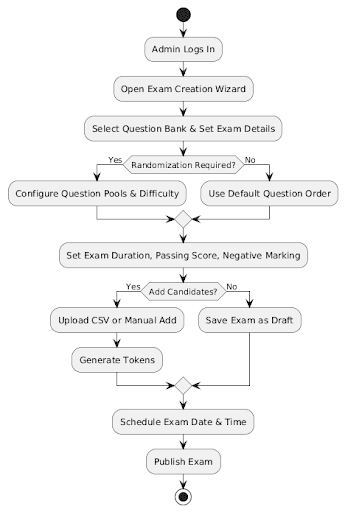
\includegraphics[width=0.7\textwidth]{assets/activity_diagrams/Exam Creation and Scheduling.png}
    \end{center}
    
    \textit{Flexible workflow supporting draft saving and immediate candidate assignment}
\end{frame}

\begin{frame}{AD: Candidate Exam + AI Proctoring}
    \begin{center}
        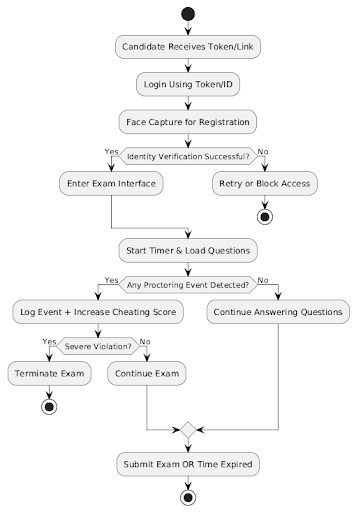
\includegraphics[width=0.65\textwidth]{assets/activity_diagrams/Candidate Exam and AI Proctoring.png}
    \end{center}
    
    \textit{Emphasizes exam integrity with real-time monitoring and violation handling}
\end{frame}

\begin{frame}{AD: Grading + Certificate Generation}
    \begin{center}
        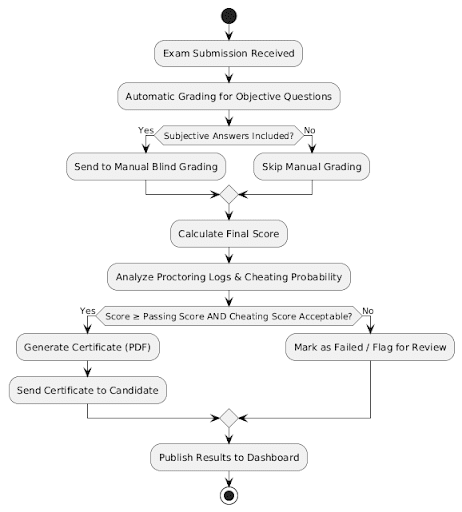
\includegraphics[width=0.7\textwidth]{assets/activity_diagrams/Grading and Certificate Generation.png}
    \end{center}
    
    \textit{Fair assessment ensuring both academic and integrity requirements}
\end{frame}

% =============================================================================
% Verification and Validation
% =============================================================================
\begin{frame}{System Model Verification \& Validation}
    \begin{block}{Requirements Validation}
        \begin{itemize}
            \item \textbf{Stakeholder Reviews:} Interactive sessions with HR managers, university administrators
            \item Confirmed requirements capture real-world needs (e.g., low-bandwidth resilience FR-CAND-005)
            \item \textbf{Prototyping:} Low-fidelity mockups validated usability requirements (FR-CAND-006)
        \end{itemize}
    \end{block}
    
    \begin{block}{Model Verification}
        \begin{itemize}
            \item \textbf{Consistency Checks:} Cross-verification between Use Case and Sequence diagrams
            \item Example: UC-08 Create Exam steps mapped to exam creation sequence diagram
            \item \textbf{Syntax Verification:} All UML diagrams verified against UML 2.5 standards
        \end{itemize}
    \end{block}
\end{frame}

\begin{frame}{Traceability Analysis}
    \begin{block}{Traceability Matrix (Sample)}
        \begin{table}[]
            \centering
            \small
            \begin{tabular}{|l|p{4cm}|p{4cm}|}
                \hline
                \textbf{Req. ID} & \textbf{Requirement Title} & \textbf{Implemented By (Use Case)} \\
                \hline
                FR-MT-002 & Enterprise Registration & UC-05: Register Enterprise \\
                \hline
                FR-MT-003 & Enterprise Account Approval & UC-01: Approve Enterprise Registration \\
                \hline
                FR-EXM-001 & Question Bank Management & UC-08: Create Exam \\
                \hline
                FR-EXM-003 & Strict Scheduling & UC-09: Schedule Exam \\
                \hline
                FR-CAND-006 & Accessibility & UC-18: Start Exam, UC-19: View Results \\
                \hline
                FR-GRAD-005 & Certificate Generation & UC-17: Receive Certificate \\
                \hline
            \end{tabular}
        \end{table}
    \end{block}
    
    \textit{Every critical requirement is addressed in system design}
\end{frame}


% =============================================================================
% SECTION 6: PROJECT PLAN
% =============================================================================
\section{Project Plan}

% =============================================================================
% Plan of Activities
% =============================================================================
\begin{frame}{Plan of Activities: Overview}
    \begin{block}{Agile Scrum Integration}
        Plan aligns with Agile Scrum methodology for flexibility and adaptability
        \begin{itemize}
            \item Iterative sprints with user-centered design
            \item Research + development integration
            \item Continuous stakeholder feedback
        \end{itemize}
    \end{block}
    
    \begin{block}{Key Phases}
        \begin{enumerate}
            \item Requirement Analysis and Research Phase
            \item System Design Phase
            \item Implementation Phase
            \item Testing Phase
            \item Documentation and Finalization Phase
        \end{enumerate}
    \end{block}
\end{frame}

% =============================================================================
% Phase 1: Requirements
% =============================================================================
\begin{frame}{Phase 1: Requirement Analysis \& Research}
    \begin{block}{Activities}
        \begin{itemize}
            \item Conduct literature review
            \item Interviews with HR managers and educators
            \item Define functional requirements
            \item Outline non-functional requirements
            \item Analyze existing tools (comparative analysis)
        \end{itemize}
    \end{block}
    
    \begin{columns}
        \column{0.5\textwidth}
        \textbf{Timeline}
        \begin{itemize}
            \item September 2025 - January 2026
            \item Duration: 4 weeks
        \end{itemize}
        
        \column{0.5\textwidth}
        \textbf{Deliverables}
        \begin{itemize}
            \item Updated requirements specification
            \item Stakeholder feedback report
        \end{itemize}
    \end{columns}
    
    \vspace{0.3cm}
    \begin{center}
        \textbf{Status:} \textcolor{green}{Completed}
    \end{center}
\end{frame}

% =============================================================================
% Phase 2: Design
% =============================================================================
\begin{frame}{Phase 2: System Design}
    \begin{block}{Activities}
        \begin{itemize}
            \item Design modular, microservices-based architecture
            \item Separate services (auth, exam, proctoring, grading, payment)
            \item Create relational database schema for system components
            \item Develop wireframes and mockups for UI/UX (Figma)
            \item Plan AI integration (facial recognition, NLP grading)
            \item Iterate designs in short sprints with team reviews
        \end{itemize}
    \end{block}
    
    \begin{columns}
        \column{0.5\textwidth}
        \textbf{Timeline}
        \begin{itemize}
            \item Late January - Early February
            \item Duration: 3 weeks
        \end{itemize}
        
        \column{0.5\textwidth}
        \textbf{Deliverables}
        \begin{itemize}
            \item System architecture document
            \item Database ER diagram
            \item UI wireframes/mockups
            \item Updated backlog
        \end{itemize}
    \end{columns}
\end{frame}

% =============================================================================
% Phase 3: Implementation
% =============================================================================
\begin{frame}{Phase 3: Implementation (1/2)}
    \begin{block}{Core Development Activities}
        \begin{itemize}
            \item \textbf{Frontend Development}
            \begin{itemize}
                \item React SPA for dashboards and exam interface
                \item Responsive design for various screen sizes
                \item Real-time updates via WebSocket
            \end{itemize}
            
            \item \textbf{Backend Development}
            \begin{itemize}
                \item Go services: API gateway, real-time proctoring event streamer
                \item Python/FastAPI: AI services (facial recognition, NLP grading)
                \item PostgreSQL database setup and optimization
            \end{itemize}
        \end{itemize}
    \end{block}
\end{frame}

\begin{frame}{Phase 3: Implementation (2/2)}
    \begin{block}{Module Development}
        \begin{itemize}
            \item \textbf{Proctoring Module}
            \begin{itemize}
                \item Tab-switch detection, mouse tracking
                \item Facial recognition with liveness detection (OpenCV/DeepFace)
                \item Cheating probability score calculation
            \end{itemize}
            
            \item \textbf{Automated Grading Module}
            \begin{itemize}
                \item Objective question auto-grading
                \item NLP-based essay grading (Transformer models)
                \item Blind grading interface for human reviewers
            \end{itemize}
            
            \item \textbf{Module Integration}
            \begin{itemize}
                \item Code reviews and sprint demos every week
                \item Continuous integration/deployment pipeline
            \end{itemize}
        \end{itemize}
    \end{block}
    
    \textbf{Timeline:} February - May 2026 (9 weeks) \\
    \textbf{Deliverables:} Code repository, API documentation, prototype demo
\end{frame}

% =============================================================================
% Phase 4: Testing
% =============================================================================
\begin{frame}{Phase 4: Testing \& Quality Assurance}
    \begin{block}{Testing Levels}
        \begin{description}
            \item[Unit Tests] PyTest (Python), Go Test (Go), Jest (JavaScript)
            \begin{itemize}
                \item Individual function and component testing
                \item Target: 95\% code coverage
            \end{itemize}
            
            \item[Integration Tests] Module interaction testing
            \begin{itemize}
                \item API endpoint testing
                \item Database transaction verification
                \item Service communication validation
            \end{itemize}
            
            \item[System Testing] Functionality, performance, non-functional aspects
            \begin{itemize}
                \item End-to-end workflow testing
                \item Security vulnerability scanning
            \end{itemize}
        \end{description}
    \end{block}
\end{frame}

\begin{frame}{Phase 4: Specialized Testing}
    \begin{block}{Scalability Testing}
        \begin{itemize}
            \item \textbf{Tool:} Apache JMeter
            \item \textbf{Target:} 500+ concurrent users on typical Ethiopian networks
            \item \textbf{Scenarios:} Peak exam load, simultaneous submissions
            \item \textbf{Metrics:} Response time, throughput, error rate
        \end{itemize}
    \end{block}
    
    \begin{block}{Security Testing}
        \begin{itemize}
            \item \textbf{Red Teaming:} Attempt to bypass proctoring
            \item \textbf{Target:} Detection rate above 95\%
            \item \textbf{Penetration Testing:} OWASP Top 10 vulnerability assessment
        \end{itemize}
    \end{block}
    
    \begin{block}{User Acceptance Testing (UAT)}
        \begin{itemize}
            \item Pilot with enterprises/candidates
            \item Feedback on usability and automated grading fairness
        \end{itemize}
    \end{block}
    
    \textbf{Timeline:} May 2026 (2 weeks) \\
    \textbf{Deliverables:} Test plans/reports, AI accuracy metrics, updated prototype, security audit
\end{frame}

% =============================================================================
% Phase 5: Documentation
% =============================================================================
\begin{frame}{Phase 5: Documentation \& Finalization}
    \begin{block}{Activities}
        \begin{itemize}
            \item Fix bugs identified from pilots
            \item Refine features based on UAT feedback
            \item Prepare comprehensive documentation
            \begin{itemize}
                \item Technical documentation (Swagger/OpenAPI for FastAPI, JSDoc for React)
                \item User manuals (including facial recognition setup)
                \item System administrator guides
                \item Local-network troubleshooting guides
            \end{itemize}
            \item Plan maintenance mechanism for updates
            \item Compile final project report
            \item Prepare defense presentation
        \end{itemize}
    \end{block}
    
    \textbf{Timeline:} May 2026 (concurrent with testing) \\
    \textbf{Deliverables:} Final system, complete documentation, project report, presentation
\end{frame}

% =============================================================================
% Timeline Overview
% =============================================================================
\begin{frame}{Timeline Overview}
    \begin{table}[]
        \centering
        \small
        \begin{tabular}{|l|p{4.5cm}|c|c|c|}
            \hline
            \textbf{Phase} & \textbf{Task/Activity} & \textbf{Start} & \textbf{End} & \textbf{Weeks} \\
            \hline
            1. Requirements & Research and gathering & 2025-10-01 & 2025-11-03 & 4 \\
            \hline
            2. Design & Architecture, database, UI & 2025-12-13 & 2026-01-07 & 3 \\
            \hline
            3. Implementation & Frontend, backend, AI integration & 2026-02-08 & 2026-04-08 & 9 \\
            \hline
            4. Testing & Unit, integration, system, UAT & 2026-04-09 & 2026-04-20 & 2 \\
            \hline
            5. Documentation & Adjustments, docs, finalization & 2026-04-01 & 2026-06-07 & 9 \\
            \hline
        \end{tabular}
    \end{table}
    
    \vspace{0.3cm}
    \textbf{Overall Milestones:}
    \begin{itemize}
        \item Prototype by March 2026
        \item Testable system by April 2026
        \item Completion by June 2026
    \end{itemize}
\end{frame}

% =============================================================================
% Risk Management
% =============================================================================
\begin{frame}{Risk Management \& Monitoring}
    \begin{block}{Identified Risks}
        \begin{description}
            \item[Technical Risks]
            \begin{itemize}
                \item Delays in module integration
                \item AI model accuracy below targets
                \item Infrastructure limitations (bandwidth, server capacity)
            \end{itemize}
            
            \item[Resource Risks]
            \begin{itemize}
                \item Team member availability
                \item Hardware/software resource constraints
                \item Budget limitations
            \end{itemize}
            
            \item[External Risks]
            \begin{itemize}
                \item Stakeholder availability for feedback
                \item Changes in regulatory requirements
                \item Third-party service dependencies (payment gateways)
            \end{itemize}
        \end{description}
    \end{block}
    
    \begin{block}{Monitoring Mechanisms}
        \begin{itemize}
            \item Agile tools: Trello for milestones, GitHub Projects for task tracking
            \item Monthly advisor reports
            \item Weekly team sprint reviews
        \end{itemize}
    \end{block}
\end{frame}

% =============================================================================
% Budget
% =============================================================================
\begin{frame}{Budget Required}
    \begin{block}{Budget Overview}
        \textbf{Total Estimated Budget: 27,000 ETB}
        
        \textit{Tailored for 9-month academic cycle (November 2025 - June 2026)}
    \end{block}
    
    \begin{table}[]
        \centering
        \small
        \begin{tabular}{|l|p{5.5cm}|r|}
            \hline
            \textbf{Category} & \textbf{Description} & \textbf{Amount (ETB)} \\
            \hline
            Connectivity & Internet/Data for cloud access and research (6 months) & 15,000 \\
            \hline
            Resources & API/Cloud Credits (OpenCV/Firebase buffers beyond free tiers) & 5,000 \\
            \hline
            Documentation & Printing \& Binding (final thesis, posters, technical docs) & 2,500 \\
            \hline
            Fieldwork & Transport for data collection and supervisor meetings & 2,000 \\
            \hline
            Contingency & Emergency buffer (10\% for hardware repairs, price fluctuations) & 2,500 \\
            \hline
            \multicolumn{2}{|r|}{\textbf{Total}} & \textbf{27,000} \\
            \hline
        \end{tabular}
    \end{table}
\end{frame}

\begin{frame}{Budget Justification}
    \begin{block}{Key Assumptions \& Cost-Saving Strategies}
        \begin{description}
            \item[Equipment] Zero-rating external HD webcams. Using built-in laptop cameras for prototype.
            
            \item[Hosting \& Software] Local demonstration or free-tier services (GitHub Pages, Heroku Free). Small API/AI credits buffer for heavy model training.
            
            \item[Internet/Data] Primary expense (60\% of budget). Critical for Git collaboration and documentation access. Ethio Telecom 10GB monthly student packages.
            
            \item[Open-Source Core] Python (OpenCV/TensorFlow), React.js eliminate licensing fees.
            
            \item[University Labs] Development and testing in university labs saves electricity and infrastructure costs.
            
            \item[Student Credits] GitHub Student Developer Pack for free tools and training.
        \end{description}
    \end{block}
\end{frame}


% =============================================================================
% CONCLUSION
% =============================================================================
\section{Conclusion}

% =============================================================================
% Summary
% =============================================================================
\begin{frame}{Project Summary}
    \begin{block}{What We've Accomplished}
        \textbf{Veritas} addresses the critical need for a secure, localized online assessment platform tailored for Ethiopian enterprises and institutions.
    \end{block}
    
    \begin{block}{Key Achievements}
        \begin{itemize}
            \item Comprehensive requirements analysis through stakeholder interviews and literature review
            \item Detailed system design with multi-tenant architecture
            \item Functional and non-functional requirements specification
            \item Complete system modeling (use cases, sequence diagrams, activity diagrams)
            \item Verification and validation of system models
            \item Detailed project plan with timeline and budget
            \item Prototype UI flow and presentation artifacts
        \end{itemize}
    \end{block}
\end{frame}

% =============================================================================
% Key Innovations
% =============================================================================
\begin{frame}{Key Innovations}
    \begin{enumerate}
        \item \textbf{Offline-Tolerant ``Passive AI'' Proctoring}
        \begin{itemize}
            \item Client-side processing reduces bandwidth requirements
            \item Tab-switch detection, periodic image capture
            \item Local face verification without continuous streaming
            \item Graceful degradation for unstable connections
        \end{itemize}
        
        \item \textbf{Automated Subjective Grading}
        \begin{itemize}
            \item NLP-based essay grading using Transformer models
            \item Reduces manual workload and human bias
            \item Blind grading interface for human review
            \item Hybrid approach: AI assistance + human oversight
        \end{itemize}
        
        \item \textbf{Data Sovereignty Compliance}
        \begin{itemize}
            \item Local hosting within Ethiopia
            \item Compliance with Personal Data Protection Proclamation
            \item Supports Digital Ethiopia 2030 Strategy
            \item Multi-tenant architecture for organizational independence
        \end{itemize}
    \end{enumerate}
\end{frame}

% =============================================================================
% Addressing the Gaps
% =============================================================================
\begin{frame}{How Veritas Addresses Literature Gaps}
    \begin{table}[]
        \centering
        \small
        \begin{tabular}{|p{3.5cm}|p{6.5cm}|}
            \hline
            \textbf{Gap Identified} & \textbf{Veritas Solution} \\
            \hline
            Security vs. Connectivity & Offline-first approach with local data queuing and periodic sync. Client-side AI processing. \\
            \hline
            Intelligent Proctoring & Accessible ``Passive AI'' with tab-switch detection, periodic image capture, local face verification. \\
            \hline
            Local Customization & Indigenous platform compliant with Ethiopian data protection laws. Amharic support. Local payment integration (Telebirr). \\
            \hline
            Accessibility & WCAG 2.1 AA compliance. Font size/contrast controls. Keyboard navigation. \\
            \hline
            ASAG \& AES & LLM-based grading with human-in-the-loop. Rubric-based evaluation. Blind grading to reduce bias. \\
            \hline
        \end{tabular}
    \end{table}
\end{frame}

% =============================================================================
% Contributions
% =============================================================================
\begin{frame}{Contributions to the Field}
    \begin{block}{Academic Contributions}
        \begin{itemize}
            \item Blueprint for resource-efficient, AI-enhanced assessment systems
            \item Demonstrates microservices architecture combining Go + Python
            \item Integration of continuous identity verification with semantic AI grading
            \item Contextual understanding beyond keyword matching
            \item Addresses trade-offs between security, privacy, and usability
        \end{itemize}
    \end{block}
    
    \begin{block}{Practical Contributions}
        \begin{itemize}
            \item Reduces dependency on foreign platforms
            \item Lowers assessment costs for Ethiopian organizations
            \item Enables scalable, fair evaluations
            \item Supports e-learning, recruitment, and certification processes
            \item Fosters technological independence in resource-constrained settings
        \end{itemize}
    \end{block}
\end{frame}

% =============================================================================
% Benefits to Stakeholders
% =============================================================================
\begin{frame}{Benefits to Stakeholders}
    \begin{columns}
        \column{0.5\textwidth}
        \textbf{For Enterprises \& HR}
        \begin{itemize}
            \item Streamlined recruitment process
            \item Reduced bias via AI grading
            \item Cost-effective (No Forex payments)
            \item Data sovereignty compliance
            \item Customizable branding
            \item Comprehensive analytics
        \end{itemize}
        
        \textbf{For Educational Institutions}
        \begin{itemize}
            \item Scalable examination platform
            \item Automated grading reduces workload
            \item Detailed performance analytics
            \item Certificate automation
        \end{itemize}
        
        \column{0.5\textwidth}
        \textbf{For Candidates}
        \begin{itemize}
            \item Fair testing environment
            \item Works on lower bandwidth
            \item Immediate feedback
            \item Transparent evaluation
            \item Accessible interface
            \item Automated certification
        \end{itemize}
        
        \textbf{For Ethiopia}
        \begin{itemize}
            \item Digital sovereignty
            \item Technological independence
            \item Local data storage
            \item Job creation (maintenance, support)
            \item Contribution to Digital Ethiopia 2030
        \end{itemize}
    \end{columns}
\end{frame}

% =============================================================================
% Challenges and Lessons Learned
% =============================================================================
\begin{frame}{Challenges \& Lessons Learned}
    \begin{block}{Key Challenges}
        \begin{itemize}
            \item Balancing security with usability and accessibility
            \item Designing for unstable network conditions
            \item AI model accuracy vs. computational efficiency trade-offs
            \item Ensuring fairness in automated grading
            \item Multi-tenant data isolation complexity
        \end{itemize}
    \end{block}
    
    \begin{block}{Lessons Learned}
        \begin{itemize}
            \item Infrastructure constraints must drive architectural decisions
            \item User-centered design is critical for adoption
            \item Hybrid approaches (AI + human) provide best results
            \item Stakeholder feedback essential throughout development
            \item Agile methodology enables adaptation to changing requirements
        \end{itemize}
    \end{block}
\end{frame}

% =============================================================================
% Future Work
% =============================================================================
\begin{frame}{Future Work \& Enhancements}
    \begin{block}{Short-Term Enhancements (6-12 months)}
        \begin{itemize}
            \item Mobile application (Android/iOS) for broader accessibility
            \item Advanced biometric authentication (fingerprint, voice)
            \item Real-time human proctoring option (video streaming)
            \item Enhanced AI models with larger, more diverse training datasets
            \item Integration with national identity systems
        \end{itemize}
    \end{block}
    
    \begin{block}{Long-Term Vision (1-3 years)}
        \begin{itemize}
            \item Large-scale government deployment for national exams
            \item Integration with university management systems
            \item Advanced analytics with predictive modeling
            \item Blockchain-based certificate verification
            \item Regional expansion to other East African countries
            \item Continuous learning AI models adapting to new cheating patterns
        \end{itemize}
    \end{block}
\end{frame}

% =============================================================================
% Recommendations
% =============================================================================
\begin{frame}{Recommendations}
    \begin{block}{For Implementation}
        \begin{enumerate}
            \item Conduct pilot programs with 2-3 partner organizations
            \item Establish dedicated support team for onboarding
            \item Develop comprehensive training materials for administrators
            \item Create feedback loop for continuous improvement
            \item Plan phased rollout to manage risk
        \end{enumerate}
    \end{block}
    
    \begin{block}{For Policy Makers}
        \begin{enumerate}
            \item Incentivize adoption of locally developed platforms
            \item Establish clear data protection regulations
            \item Support research in AI ethics and fairness
            \item Invest in digital infrastructure improvements
            \item Promote public-private partnerships for technology development
        \end{enumerate}
    \end{block}
\end{frame}

% =============================================================================
% Impact Assessment
% =============================================================================
\begin{frame}{Expected Impact}
    \begin{block}{Quantitative Impact}
        \begin{itemize}
            \item \textbf{Cost Reduction:} 60-70\% savings compared to foreign platforms
            \item \textbf{Time Savings:} 80\% reduction in subjective grading time
            \item \textbf{Scalability:} Support 500+ concurrent users per exam
            \item \textbf{Accuracy:} Target 95\% cheating detection rate
            \item \textbf{Efficiency:} Automated certificate generation within minutes
        \end{itemize}
    \end{block}
    
    \begin{block}{Qualitative Impact}
        \begin{itemize}
            \item Enhanced trust in online assessments
            \item Improved fairness and reduced bias
            \item Greater accessibility for diverse user groups
            \item Strengthened digital sovereignty
            \item Contribution to technological independence
        \end{itemize}
    \end{block}
\end{frame}

% =============================================================================
% Alignment with Digital Ethiopia 2030
% =============================================================================
\begin{frame}{Alignment with Digital Ethiopia 2030 Strategy}
    \begin{block}{Strategic Alignment}
        \textbf{Digital Ethiopia 2030 Pillars:}
        \begin{description}
            \item[Digital Sovereignty] $\checkmark$ Local data storage, indigenous platform development
            \item[Digital Infrastructure] $\checkmark$ Optimized for Ethiopian network conditions
            \item[Digital Skills] $\checkmark$ Training for administrators, support job creation
            \item[Digital Services] $\checkmark$ E-learning, recruitment, certification services
            \item[Digital Innovation] $\checkmark$ AI integration, microservices architecture
        \end{description}
    \end{block}
    
    \vspace{0.3cm}
    \begin{center}
        \textit{Veritas directly supports Ethiopia's vision for technological independence and digital transformation}
    \end{center}
\end{frame}

% =============================================================================
% Final Thoughts
% =============================================================================
\begin{frame}{Final Thoughts}
    \begin{block}{Project Significance}
        Veritas represents more than just an assessment platform—it's a step toward:
        \begin{itemize}
            \item \textbf{Technological Independence:} Reducing reliance on foreign solutions
            \item \textbf{Educational Equity:} Providing fair, accessible evaluation tools
            \item \textbf{Economic Empowerment:} Keeping resources within Ethiopia
            \item \textbf{Innovation Leadership:} Demonstrating local capacity for complex systems
        \end{itemize}
    \end{block}
    
    \begin{block}{Moving Forward}
        The foundation has been laid through:
        \begin{itemize}
            \item Comprehensive requirements analysis
            \item Robust system design
            \item Detailed implementation plan
            \item Clear roadmap for future enhancements
        \end{itemize}
    \end{block}
    
    \vspace{0.3cm}
    \begin{center}
        \textbf{Next step: Implementation and validation through prototype development}
    \end{center}
\end{frame}

% =============================================================================
% Thank You
% =============================================================================
\begin{frame}{Thank You}
    \begin{center}
        
\includegraphics[width=3cm]{assets/aastu_logo.jpg}
        
        \vspace{1cm}
        
        {\Large \textbf{Veritas: AI Enhanced Online Assessment and Monitoring System}}
        
        \vspace{0.5cm}
        
        {\large \textbf{Thank You for Your Attention!}}
        
        \vspace{1cm}
        
        \textbf{Questions \& Discussion}
        
        \vspace{0.5cm}
        
        \textit{Team Veritas} \\
        Department of Software Engineering \\
        Addis Ababa Science and Technology University
    \end{center}
\end{frame}

% =============================================================================
% Backup Slides
% =============================================================================
\appendix

\begin{frame}{Backup: Technology Stack Details}
    \begin{columns}
        \column{0.5\textwidth}
        \textbf{Backend}
        \begin{itemize}
            \item Go 1.21+
            \item Python 3.11+
            \item FastAPI framework
            \item PostgreSQL 15+
            \item Redis (caching)
            \item RabbitMQ (message queue)
        \end{itemize}
        
        \textbf{AI/ML}
        \begin{itemize}
            \item OpenCV
            \item DeepFace
            \item Transformers (HuggingFace)
            \item TensorFlow/PyTorch
        \end{itemize}
        
        \column{0.5\textwidth}
        \textbf{Frontend}
        \begin{itemize}
            \item React 18+
            \item TypeScript
            \item Material-UI
            \item WebSocket (Socket.io)
            \item IndexedDB
        \end{itemize}
        
        \textbf{DevOps}
        \begin{itemize}
            \item Docker
            \item Kubernetes
            \item GitHub Actions (CI/CD)
            \item Prometheus (monitoring)
            \item Grafana (visualization)
        \end{itemize}
    \end{columns}
\end{frame}

\begin{frame}{Backup: Security Measures}
    \begin{itemize}
        \item \textbf{Authentication:} JWT tokens with refresh mechanism
        \item \textbf{Authorization:} Role-based access control (RBAC)
        \item \textbf{Encryption:} TLS 1.2+ for transit, AES-256 for rest
        \item \textbf{Password Security:} bcrypt hashing with salt
        \item \textbf{API Security:} Rate limiting, input validation, CORS
        \item \textbf{Database Security:} Parameterized queries, least privilege access
        \item \textbf{Audit Logging:} Immutable logs for all critical operations
        \item \textbf{Compliance:} OWASP Top 10, PCI DSS Level 2
    \end{itemize}
\end{frame}

\end{document}


\end{document}
